

\chapter{Techniques of Interferometry}
\minitoc

\pg
In this section, we contextualise the work done as part of this PhD by discussing the difficulties introduced by the combination of sparse $uv$-coverage and weak \emph{a priori} constraints on the sky brightness distribution. The conceptual framework which we rely on throughout this manuscript, the Radio Interferometer's Measurement Equation, is described in greater detail in  \cref{section.RIME}. We will begin by discussing radio interferometry itself. We will then discuss the so-called \emph{imaging problem}, and end by discussing the \emph{calibration problem}. Note that both of these are artifical subsets of the general inverse problem of radio interferometry. While in practice calibration is done before imaging, it is conceptually helpful to begin with imaging. Until we reach our introduction to radio interferometric calibration, we will therefore assume that calibration has been successfully carried out, and that we are working on the \emph{corrected visibilities}, i.e. gain-corrected visibilities. 

\pg
We start by linking interferometry to more concrete concepts: specifically, we will give a (very!) brief introduction to radio antennas and their characteristics. We will then use this introduction to show the advantages and drawbacks of radio interferometry, along with the concrete technical problems that the method introduces.

% will make the ideas and basis of radio interferometry more accessible by allowing us to explain the abstractions that interferometry relies on in terms of simpler instrumental configurations. We will then introduce the concrete problems that interferometry introduces: both a recapitulation of the venerable Zernike-van Cittert theorem \citep[cf.][]{1934Phy.....1..201V} and the problem of incomplete $uv$-cove	rage.



\clearpage
% !TeX spellcheck = en_UK


%
%\pg
%There exists a wide variety of methods used in imaging, from the venerable CLEAN algorithm\footnote{For an excellent beginner's introduction to CLEAN, the author heartily recommends \url{https://www.cv.nrao.edu/~abridle/deconvol/node7.html}} to cutting-edge compressed sensing and subspace deconvolution methods. We will begin this section by introducing a mathematical framework in which the problem of deconvolution can be understood, and proceed, from there, to discuss some of the deconvolution algorithms which can be used.
%
%\pg
%The formalism used in this section is based, in part or in whole, on that used by Cyril Tasse in [DDF paper].

\section{A Brief Introduction to Radio Astronomy}
\pg
Radio astronomy consists of observing the electromagnetic emission of astrophysical\footnote{And, famously, attempting to observe ``intelligent" sources \citepads[cf]{2017AAS...22911604E}} sources at very long wavelengths by means of radio antennas. These antennas measure a voltage proportional to variations in the electromagnetic field in all the directions they are sensitive to. Since astrophysical signals are weak, a good sensitivity is necessary. Achieving good sensitivity with radio antennas means having a very large collecting area - in this respect, they behave exactly the same way as optical telescopes. Similarly, when well-designed, they are diffraction-limited - this means that, once again like optical telescopes, their resolution is limited by their diameter.

\pg
However, because radio frequencies are so much lower, achieving a resolution comparable to e.g. the HST requires extremely large dishes. While there exist telescopes, both old and new, which work on this principle (from Arecibo Observatory, shown in \cref{fig.arecibo}, to the upcoming FAST telescope in China, shown in \cref{fig.FAST}), the associated technical difficulties (pointing is complex business, as are the associated optics requirements; maintenance costs are high, etc...) have made the single-dish approach prohibitive.

\begin{figure}[ht]
\centering
\begin{subfigure}{.48\textwidth}
\resizebox{\hsize}{!}{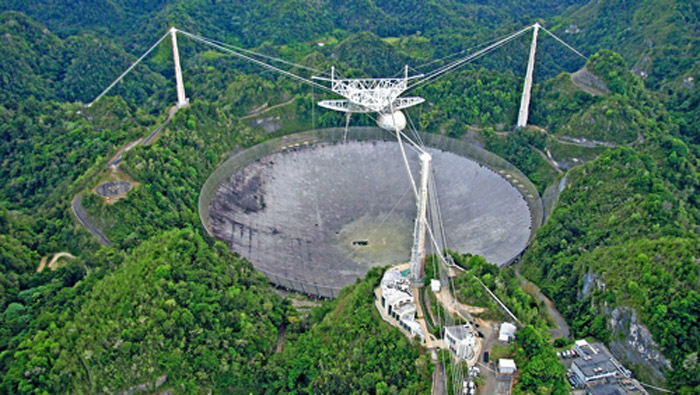
\includegraphics{images/20151101114231-0_8e7cc_c7a44aca_orig.jpg}}
\caption{\label{fig.arecibo} Arecibo telescope, in Puerto Rico.}
\end{subfigure}
\hfill
\begin{subfigure}{.48\textwidth}
\resizebox{\hsize}{!}{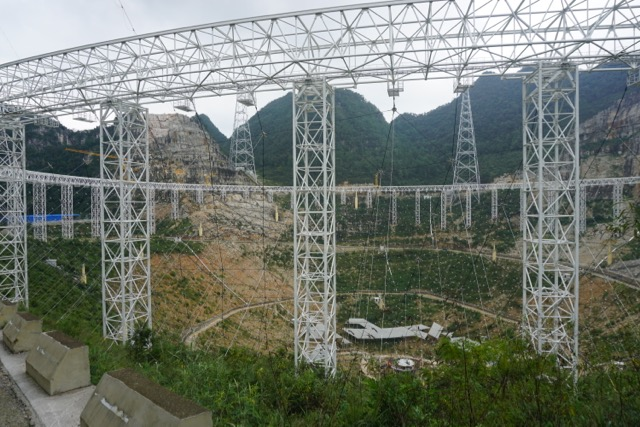
\includegraphics{images/FastTelescope_8sep2015.jpg}}
\caption{\label{fig.FAST} FAST telescope, in China}
\end{subfigure}
\caption{\label{fig.singleDishes} Examples of large single-dish radio telescopes.}
\end{figure}

\pg
One way to move past this technical limitation is to resort to interferometry: this is the topic of this section.





\section{Interferometry: Bypassing the Diffraction Limit}

\pg
There are two quantities of interest to all astronomers: sensitivity and angular resolution\footnote{Other kinds of resolution - in time and frequency, for example - are also extremely important to many astronomers, but are not what concern us here.}. An instrument's sensitivity is a function of its collecting area\footnote{It is also a function of technological factors, of course, but \emph{ceteris paribus}, a more sensitive telescope means a telescope with a wider collecting area}. Resolution, for well-designed instruments\footnote{By this, we mean that we assume that an instrument is also designed to optimise resolution.}, is limited by diffraction in the absence of atmospheric effects. This introduces specific issues in the radio domain. Radio waves have very long wavelengths - often comparable to meters, rather than the $\sim100-1000$nm wavelengths of optical light. Achieving a resolution comparable to those of optical telescopes would thus require making telescopes with apertures tens of millions of times larger than those already titanic instruments!

\pg
In practice, this technical constraint on resolution is one that astronomers are very interested in overcoming. This technical limitation therefore demands a technical solution. In practice, this solution consists of recourse to interferometric techniques. Indeed, interferometry can be thought of as the construction of a "sparse" dish, as illustrated in \cref{fig.aperture.synthesis}.

\begin{figure}[ht]
\centering
\begin{subfigure}{.43\textwidth}
\resizebox{\hsize}{!}{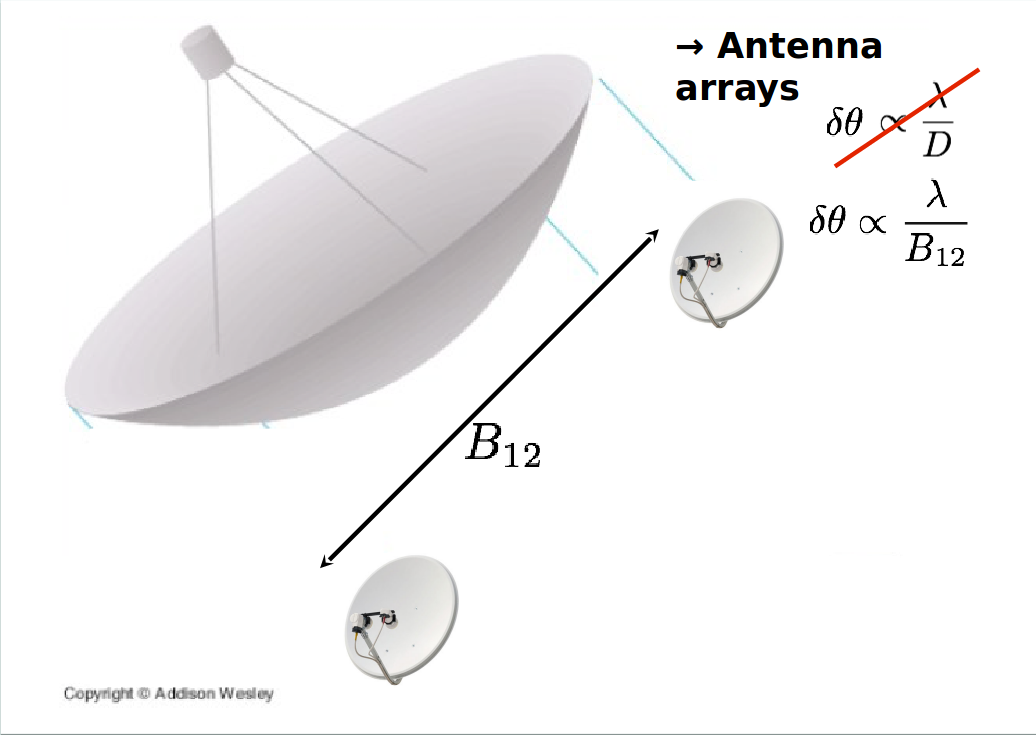
\includegraphics{images/baseline-resolution.png}}
\caption{\label{fig.baseline.image} A pair of dishes can surpass the resolution limit of its components.}
\end{subfigure}
\hfill
\begin{subfigure}{.43\textwidth}
\resizebox{\hsize}{!}{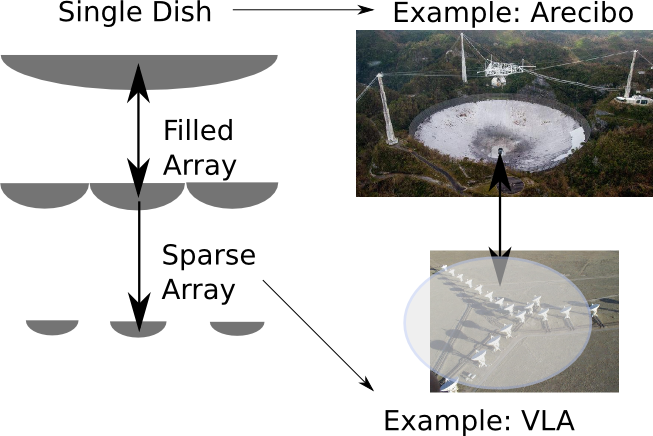
\includegraphics{images/sparseArray.png}}
\caption{\label{fig.arecibo.vla} With enough pairs of dishes, it is possible to synthesise a much larger dish.}
\end{subfigure}
\caption{\label{fig.aperture.synthesis} Illustration of the underlying principle of interferometry. The 27 dishes of the VLA can be thought of as "synthesising" a similar circular dish as Arecibo. This idea is the reason why radio interferometry is historically known as "aperture synthesis" in the literature of radio astronomy. \cref{fig.baseline.image} is copyrighted by Addison Wesley.} % \textcolor{red}{CHANGE FIG B. AS THE ELLIPSE IS NOT SEE-THROUGH}}
\end{figure}

\pg
Interferometric measurements are made as follows: the elements of the interferometric array (which can be single dishes or phased arrays\footnote{Described in \cref{sec.visibility}} of smaller antennas) measure a voltage. This voltage is correlated between antennas, as will be described shortly. Each of these correlations correspond to a single Fourier mode of the sky, as per the Zernike-van Cittert theorem (cf. \cref{sec.imag.psf}). They must be calibrated, by comparing the observations of a calibrator source and modelled visibilities. Calibration is described in much greater detail in \cref{section.RIME}. Then, the calibrated visibilities are used to reconstruct an image of the sky, which often requires deconvolution due to the sparsity of interferometric arrays.

\pg
The resolution improvement of interferometers does thus not come for free. To better understand the cost of interferometry, we will cover calibration after explaining the particularities of interferometers. We will begin with the properties of their core component: the baseline.

\subsection{The Baseline}

\pg
To define the baseline, we must begin by considering the geometric properties of an interferometric array. For now, let us assume that we are observing the sky above the array, a practice known as drift-scanning. A baseline then consists of the vector subtraction of the positions, in 3-dimensional space, of its two constituent antennas. Note that each antenna pair therefore has 2 corresponding baselines, since for each pair of antennas A and B we create baselines AB and BA. These distance vectors are then divided by the observing wavelength to give a dimensionless set of coordinates, known as $(u,v,w)$. These coordinates define the baseline entirely. 

\subsection{The Visibility}\label{sec.visibility}

\pg
We have defined what a baseline corresponds to: a vector coordinate in $(u,v,w)$-space. To each baseline we associate a measurement, which we call the \emph{visibility}. 
\begin{figure}[ht]
\centering
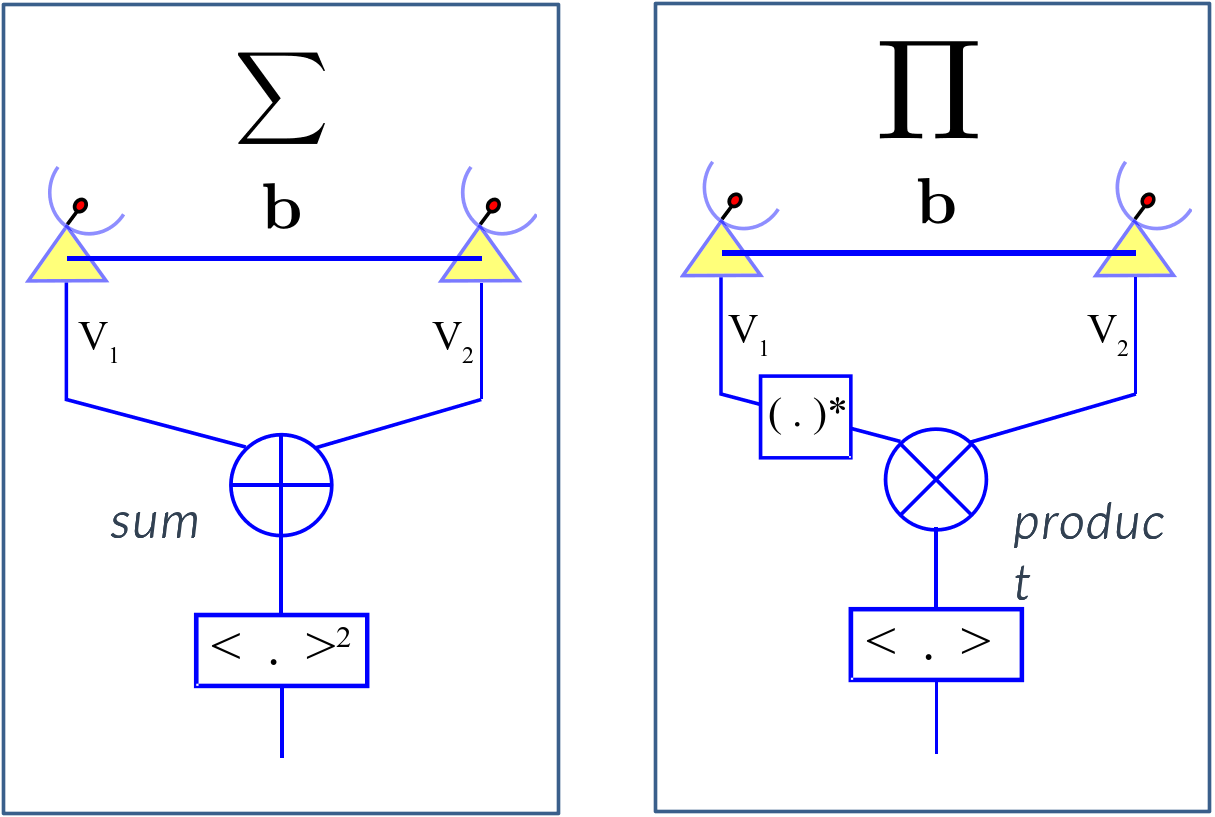
\includegraphics[width=.7\textwidth]{images/visibility-creation.png}
\caption{\label{fig.visibility} There are two ways to combine the voltages from two antennas into a visibility: they are sum-correlation and $\pi$-correlation. In this manuscript, we will only concern ourselves with the latter. Image credit: Julien Girard}
\end{figure}
The visibility associated with baseline $\mathbf{b}_{AB}$ is created by taking the voltage $V_A$ measured by antenna A, multiply it by the complex conjugate $V_B^*$ of the voltage measured by antenna B, average over the correlator dump time (i.e. the time over which the measurement is made). This scalar quantity is associated to the baseline position vector $\mathbf{b}_{AB}$. In other words:
\begin{align}
\mathbf{b}_{AB} &= \frac{\mathbf{x}_{B}-\mathbf{x}_{A}}{\lambda_\mathrm{obs}}\\
V_{AB}          &= \langle V_{A} V_{B}^*\rangle_{\delta t, \delta \nu} 
\end{align}
where $\langle \cdots \rangle_{i}$ denotes an averaging over quantity $i$. We see that a visibility is a complex vector quantity. We also see that $\mathbf{b}_{AB} = \mathbf{b}_{BA}^*$: the information of the visibility associated with baseline BA is contained in the visibility associated with baseline AB. This means that in practice, only half of the visibilities ever need be stored. What does the visibility measurement correspond to?
\begin{figure}[ht]
\centering
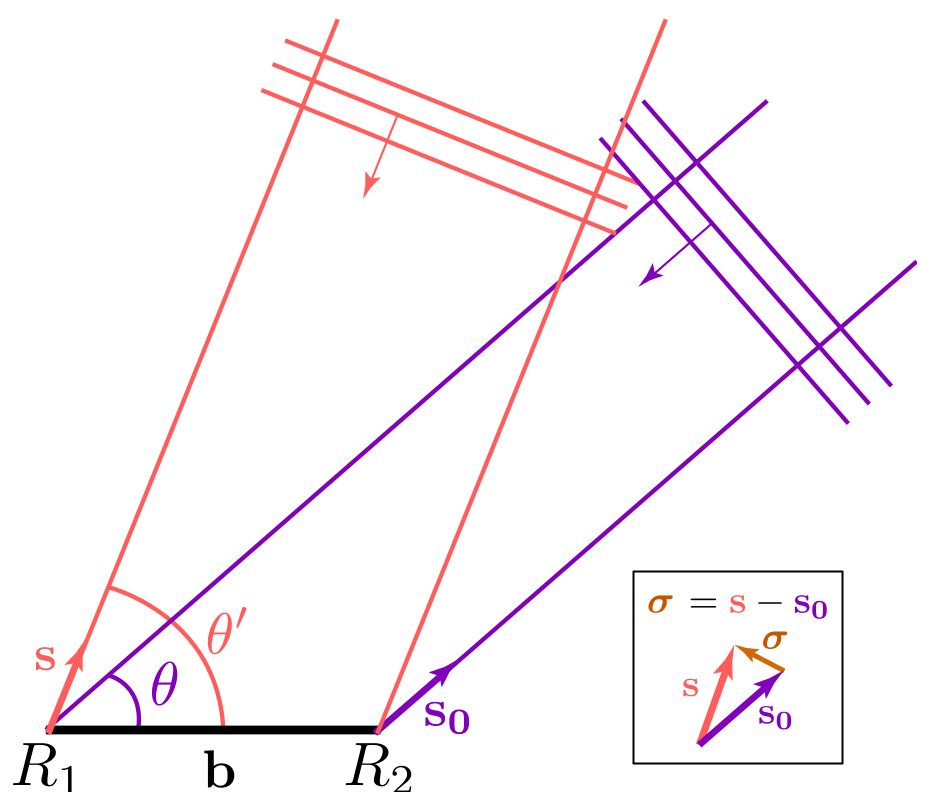
\includegraphics[width=.5\textwidth]{images/visibility-measure.png}
\caption{\label{fig.visibility.measure} Here, we assume that there are only two sources in the sky whose signal can be measured by our antennas. The final visibility is the sum of the visibilities associated with each individual source. Image credit: Julien Girard \citepads{julien}}
\end{figure}

\pg
The signals from different astrophysical do not interfere. They are measured additively in both antennas. Provided that the signal from each sources is coherent when observed by the dishes, the correlation between the voltages measured by antennas A and B will simply be the sum of the voltage correlations associated with individual sources. This is shown in \cref{fig.visibility}: the radio signal from two different sources, at two different locations, is picked up simultaneously by both radio antennas. Because only the correlation between both antennas is measured, the signals do not interfere: if the signal from each source gives a voltage $V_{p}^s$ for antenna $p$, then the additive property of electric fields means that the total visibility measured by baseline $pq$ can be written as:
\begin{align}
V_{pq}  &= \langle \left(\sum_{s} V_{p}^s\right) \left(\sum_{s} (V_{q}^s)\right)^*  \rangle_{\Delta t} \\
        &= \langle \sum_{s,s'} V_{p}^s (V_q^{s'})^*  \rangle_{\Delta t}\\
        &= \langle \sum_s V_{p}^s (V_q^{s})^* \rangle_{\Delta t} + \underbrace{\langle \sum_{s,s'\ne s} V_{p}^s (V_q^{s'})^* \rangle_{\Delta t}}_{=0} \label{eq.spatial.incor}
\end{align}
where the fact that signal from different sources is not coherent means that we average out cross-contributions (i.e. signal from $s\ne s'$). 
%\begin{align}
%V_{pq}&=\langle \left(\sum_{s} V_{p}^s\right) \left(\sum_{s} V_{q}^s \right)^* \rangle_{\Delta t} \right)\\
%      &=\langle\sum_{s,s'} \left( V_p^s\left(V_q^{s'}\right)^* \rangle_{\Delta t}
%\end{align}

\pg
Note that in Fig. \ref{fig.visibility.measure}, neither source is at the zenith. This introduces the notion of the \emph{effective baseline} which is shorter than the \emph{physical baseline} when measuring a signal from a source that is not at the zenith. Sources in different positions in the sky will be measured by an interferometric array, but the same array will have different effective baselines for different sources. To point an interferometric array in a specific direction in the sky, one must introduce a phase delay in each antenna (or, for fundamental interferometer elements such as the LOFAR tiles or NenuFAR, by playing with the cable length between each dish and the correlator). This is done by three means: delay tracking (which is exact only for the delay tracking centre\footnote{Source: \url{http://www.astron.nl/eris2013/Documents/2_laing_fundamentals_interferometry.pdf}, \url{https://science.nrao.edu/science/meetings/2016/15th-synthesis-imaging-workshop/SISS15Advanced.pdf}}, and corresponds to playing with the cable length between antennas in the interferometric array), antenna pointing\footnote{This maximises antenna sensitivity in a given direction, but is not done with LOFAR}, and fringe stopping\footnote{Fringe stopping consists of down-converting the signal received by antennas by mixing with a local oscillator. The geometric delay compensation is usually applied on this down-converted signal. Source: \url{http://www.gmrt.ncra.tifr.res.in/gmrt_hpage/Users/doc/WEBLF/LFRA/node74.html}}.
%Fringe stopping consists of measuring the beat between a predicted fringe rate (i.e. the period of the visibility sine wave corresponding to a point source out of phase centre; if the position of an array's antennas is well-known, this can be modeled accurately) and a known signal, e.g. the actual fringe rate (i.e. the fringe rate corresponding to the true period of the visibility sine wave). The difference between the two is a function of how well the antennas' positions are known. If they are well-known, then the phase information can still be measured, even without very fine sampling in time. } must be used to avoid taking a measurement every few milliseconds. 
This means that there are actually three different ``field centres", which are usually (but not always) set to be the same: the pointing (direction of maximum antenna sensitivity), the delay (which can be introduced in cable length) and the phase tracking (which consists of applying a known signal to the measured signal and recording the resulting heterodyne wave so as to keep a reasonable amount of post-correlation data without losing information on sources outside of the phase delay centre). The position of sources are then given in terms of the cardinal angle $\sigma$: this is the difference between the position of a source and the phase centre, which is where the array is pointing. For example, in \cref{fig.visibility.measure}, if we point antennas and introduce phase delays such that we are pointing the array towards Source 2, the position of Source 1 will be $\sigma$.


\subsection{The $uv$-plane}

\pg
%In general, interferometric design is such that the $w$ component of visibilities' $(u,v,w)$ coordinates is negligible (or can be put in a frame of reference where it can usually be approximated as such). 
For the sake of brevity, radio astronomers tend to talk of a $uv$-plane rather than $uvw$-space to describe visibility space. The set of $uvw$-values for all the baselines of an interferometric array is known as its $uv$-coverage, and defines the array's properties entirely.
For the VLA, for example, the instantaneous $uv$-coverage when observing the zenith will be as shown in Fig. \ref{fig.vla.uvcoverage}.

\begin{figure}[ht]
\centering
\resizebox{\hsize}{!}{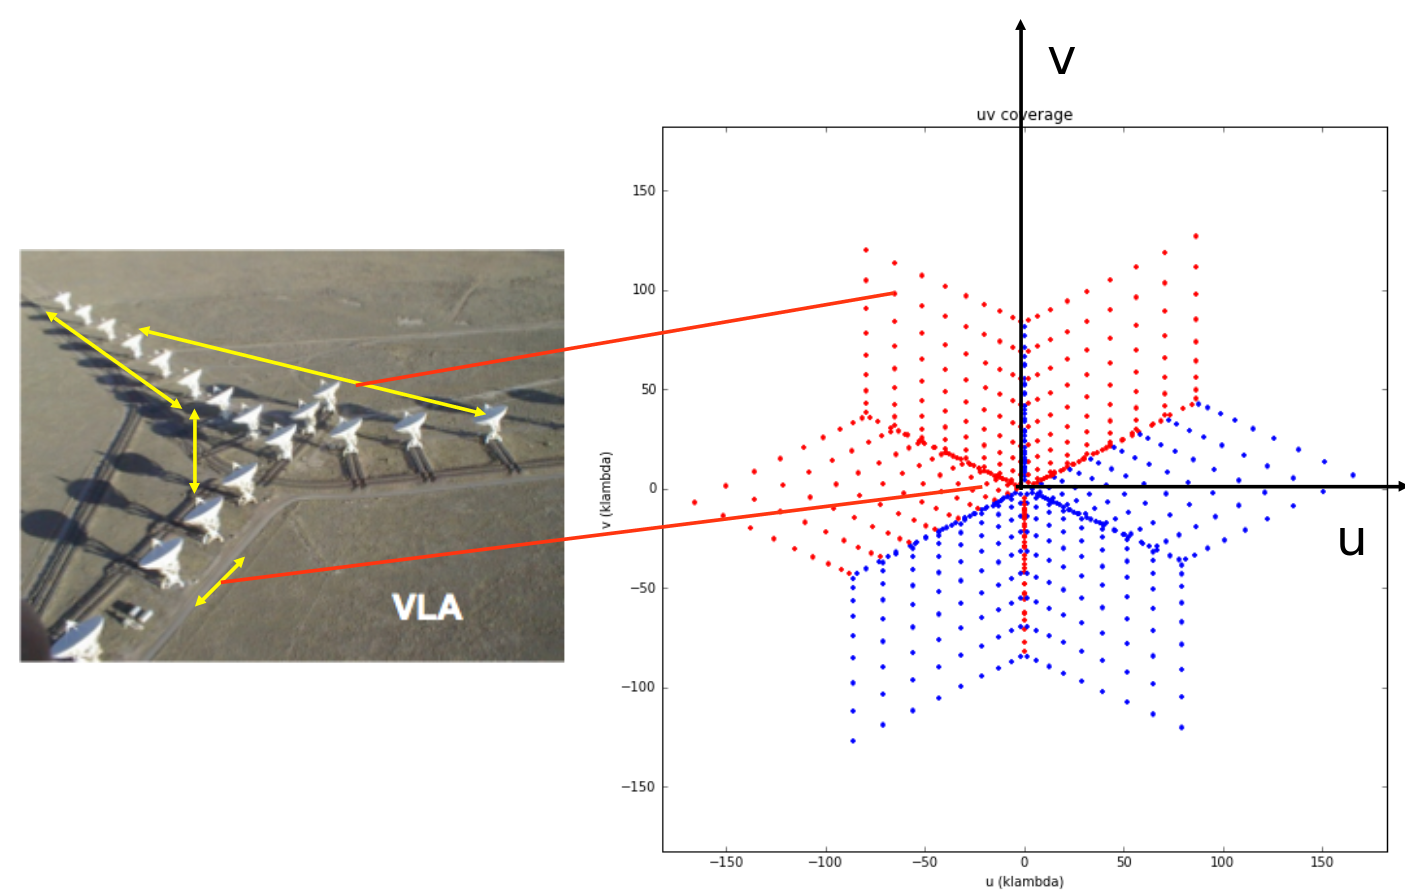
\includegraphics{images/vla-uvcoverage.png}}
\caption{\label{fig.vla.uvcoverage} The VLA contains 27 radio dishes placed as shown above. Each antenna pair between those 27 gives two single baselines, here, one red and one blue. Image credit: Julien Girard}
\end{figure}

%\pg
%The more points an array has in $uv$-space, the greater its $uv$-coverage and the better it will observe. This coverage can be improved for free in two main ways: firstly, the use of a technique known as supersynthesis (since the interferometer "synthesises" a dish at any given time, by assuming that the sky does not evolve over a certain time frame, we can treat different times as measurements of the same sky) and taking advantage of the frequency-dependence of $uv$-coordinates.The impact of both practices will be described in greater detail in \ref{sec.imag.psf}, but know that "$uv$-tracks" simply correspond to the $uv$-coverage of an interferometer observing over some period of time.

\pg
Individual antennas of an array can be pointed mechanically, and so the loss of antenna sensitivity in the direction of interest (and therefore the loss of net interferometric array sensitivity) can be minimised. But what happens to the array itself? It is useful here to go back to the illustration of Fig. \ref{fig.arecibo.vla}. Think of each dish in the array representing a "filled" segment of a massive but empty dish. By projecting our observation in a given direction, this dish goes from circular to elliptical.
\begin{figure}[ht]
\centering
\begin{subfigure}{.40\textwidth}
\resizebox{\hsize}{!}{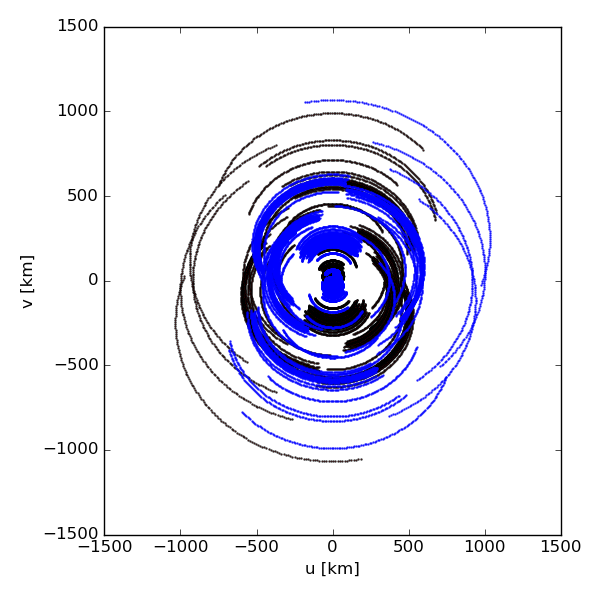
\includegraphics{images/lofar-uvcoverage-zenith.png}}
\caption{\label{fig.lofar.uvcoverage.zenith} $uv$-coverage of an 8-hour LOFAR observation when pointing at zenith.}
\end{subfigure}
\hfill
\begin{subfigure}{.40\textwidth}
\resizebox{\hsize}{!}{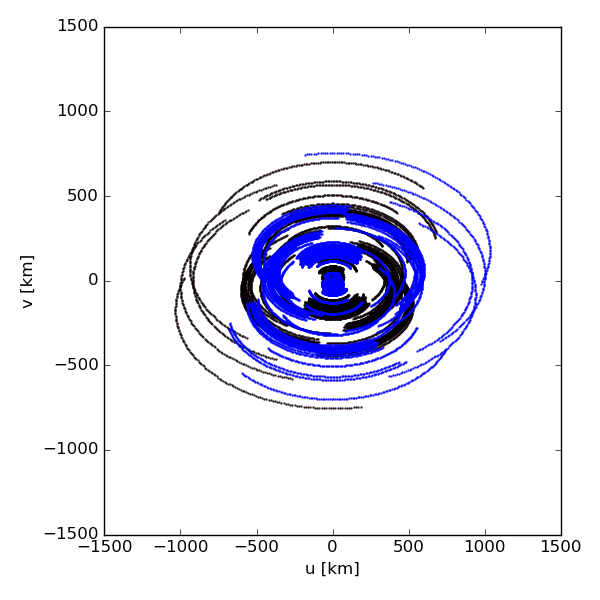
\includegraphics{images/lofar-uvcoverage-elsewhere.png}}
\caption{\label{fig.lofar.uvcoverage.elsewhere} $uv$-coverage of an 8-hour LOFAR observation when pointing 45 degrees away from zenith.}
\end{subfigure}
\caption{\label{fig.uvcoverage.lofar} Effect of array pointing on $uv$-coverage. By pointing the array 45 degrees in the $v$-axis, the array's $uv$-coverage (and thus maximum resolution) is decreased along the $v$-axis. Two colours are used, because $V_{AB}=V_{BA}$, and so only half the visibilities are stored in practice.}
\end{figure}


\subsection{The Point-Spread Function}\label{sec.imag.psf}

\pg
We have seen that the purpose an interferometric array is to overcome the diffraction limit of single-dish antennas. We have described visibilities, which are the quantities measured by an interferometric array. What remains is to describe how these measurements are related to the sky brightness distribution.

\pg
Assuming that all the antennas in an array are equivalent and perfectly calibrated, the van Cittert-Zernike theorem (\citetads{1934Phy.....1..201V}, covered in \citetads{2001isra.book.....T}) allows us to equate a visibility with a single Fourier mode of the plane tangent to the sky where the instrument is pointed. This direction is called the \emph{phase centre}, because phase shifts are introduced between antenna voltages before averaging so as to point each visibility in this direction. This behaviour is encoded in the Fourier kernel, which is written as:
\begin{equation}
k_p=2\pi i (( u_p l + v_p m + w_p (n-1) ))
\end{equation}



\pg
The Point-Spread Function (PSF) of an instrument is its point source response: it will determine the angular resolution limit due to the instrument. We know that the Fourier transform of a single point source with unit flux at phase centre is a constant. If we measured the full (infinite) visibility space, then we could reconstitute a point source perfectly. In practice, however, we only ever measure a subset of the visibility space: an interferometric array's PSF is thus the inverse Fourier transform of the array's $uv$-coverage, as these are the only points for which we have information on visibility space. The more elements in the array, the better the $uv$-coverage and thus the better the PSF. An interferometer's PSF will always be worse than an antenna dish of equivalent diameter, the UV-coverage of which is the inverse Fourier transform of a disc. This is because an interferometer behaves like a \emph{sparse} dish: the sparsity of our coverage manifests as very large point-spread function. The more baselines are available, the less sparse the UV-coverage, and so the better the PSF. This is shown in Fig. \ref{fig.vla.PSFvsUVcov}.

\pg
Mathematically, the $uv$-coverage of an interferometer can be treated as a series of delta functions centred on the antenna positions. To go from visibility space to image space, we apply the inverse Fourier transform, giving us:
\begin{align}
\mathbf{S}_{\mathrm{obs}} &= \mathcal{F}^*\left[ \mathbf{B} \sum_i^{n} \mathbf{x}_i \right]
\end{align}
where $\mathbf{S}_{\mathrm{obs}}$ is the observed sky brightness distribution, $\mathbf{B}$ the Fourier transform of the true sky brightness distribution $\mathbf{S}$, and $n$ is the number of antennas in our array. $\mathcal{F}^*$ is the inverse Fourier transform. By using the convolution theorem, we immediately see that
\begin{align}
\mathbf{S}_{\mathrm{obs}} &= \underbrace{\mathcal{F}^*\left[ \mathbf{B}\right]}_{=\mathbf{S}} \star \underbrace{\mathcal{F}^*\left[\sum_i^{n}\mathbf{x}_i \right]}_{\text{the PSF}}\\
\end{align}
and that our image is the convolution of the ``true", underlying sky brightness distribution, and our array's PSF. As $n \rightarrow \infty$, the $uv$-plane fills, and the inverse Fourier transform of this unit plane becomes 1. This illustrates the description above.

\begin{figure}[h!]
\centering
\resizebox{\hsize}{!}{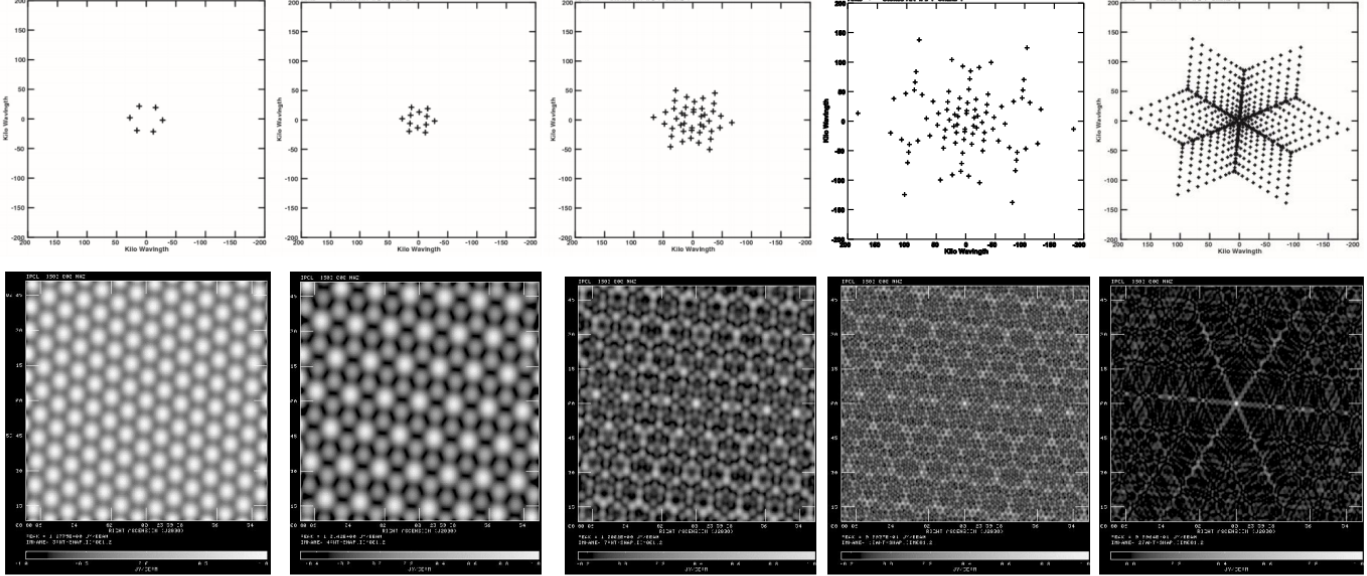
\includegraphics{images/PSFvsUVcov.png}}
\caption{\label{fig.vla.PSFvsUVcov}Plot of the PSF associated to more and more complete UV-coverage (here, consisting of more and more elements of the VLA). Image credit: Rick Perley, 3GC4 lecture.}
\end{figure}

\pg
This PSF can be improved by assuming that the sky is constant over periods of time (supersynthesis) or constant over fractions of the total bandwidth. This improves UV-coverage by a factor $N_\mathrm{t}\times N_\nu$, the number of measurements in time and frequency respectively. The effect of supersynthesis on the PSF is shown in Fig. \ref{fig.vla.PSFsupersynthesis}.
\begin{figure}[h!]
\centering
\resizebox{\hsize}{!}{\includegraphics{images/{PSF_supersynthesis}.png}}
\caption{\label{fig.vla.PSFsupersynthesis}Effect of supersynthesis on the UV-coverage of the full VLA. Image credit: Rick Perley, 3GC4 lecture.}
\end{figure}

\pg
Of course, even with these techniques, the PSF is never perfect, and flux from very bright sources will contaminate the rest of the field. The source in the last image of Fig. \ref{fig.vla.PSFsupersynthesis}, for example, only appears point-like by contrast to the others. If we wish to recover faint emission - and when interested in deep extragalactic fields, that is exactly what we wish to do - then we need to ensure that the effect of the PSF in our images is mitigated, for the brighter sources at least, lest their sidelobes (tails of the PSF convolved with the source) drown out signal from fainter sources. This means \emph{deconvolving} the PSF from radio interferometric images.

\subsection{From Dirty to Clean: Deconvolving the PSF}\label{section.clean}

\pg
Raw images made from radio interferometric data consist of the underlying flux distribution convolved to the array's PSF. The quantity of interest to astronomers is the underlying flux distribution. To recover that information from images, deconvolution is needed.

\pg
In practice, performing a full deconvolution on large images (easily over 25 million pixels in total) is not computationally viable. Scientists therefore resort to algorithms and techniques to accelerate imaging and deconvolution. For example, the use of Direct Fourier Transforms (DFT), which are extremely slow, is avoided when going from visibility space to image space - Fast Fourier Transforms (FFTs) are preferred. Similarly, one seeks to avoid having to perform full deconvolution on the dirty image, since many pixels in the image do not actually contain astrophysical signal. In this chapter, we will briefly cover the most common method of deconvolution used in radio astronomy.

\pg
We use dynamic range (DR) as a quality metric in radio images. DR is the ratio of the flux of the brightest source in the field to the flux of the faintest source in the field detectable above the noise. It is therefore a function of both source brightness and noise, and so we define dynamic range as:
\begin{equation}\label{eq.DR.imag}
DR = \frac{S_{max}}{\max(S_{min},\sigma)}
\end{equation}
where $S_{max}$ is the flux of the brightest source in the image, $S_{min}$ the flux of the faintest source detectable above the noise, and $\sigma$ is the noise in the image. The higher the DR, the deeper we image the sky, and thus the better the image. There are two big constraints to reckon with: firstly, we do not want to deconvolve the PSF from all pixels in the image, but only from those within which large amounts of underlying flux fall. Secondly, if we only deconvolve some pixels rather than performing a full deconvolution, then care must be taken not to treat artefacts in the field (which can be created from overlapping PSF sidelobes from neighbouring sources, even with perfect calibration) as true flux. Doing so would lead to an attempt to deconvolve a PSF from a pixel while assuming an incorrect underlying flux value for this pixel and thus result in the introduction of further artefacts in the image.


\pg
The dominant family of deconvolution algorithms used in radio astronomy at the time of writing is CLEAN\footnote{The other main family of deconvolution algorithms, Maximum Entropy Methods (MEM), are not very widely-used at the time of writing, but remain an active area of research (cf. \citetads{2018ApJ...857...23C}).} \citepads[see]{1974A&AS...15..417H,1984ARA&A..22...97P}, which is understood in compressed sensing theory as a matching-pursuit algorithm optimising L2 (i.e. a least-squares fit) with the addition of an L1 regularisation (i.e. the total flux in the model is minimised). The various CLEAN algorithms seek out the brightest pixel(s) in the image, potentially applying a mask to the image first in cases where some \emph{a priori} knowledge on flux distribution is available. It then deconvolves those pixels up to a predefined threshold (either a fraction of the initial pixel value or some factor of the estimated noise value). It does this some predefined number of times. Then, it collects the aggregate \emph{model} (the flux estimate for each deconvolved pixel up to this point), convolves the model with the PSF, and subtracts the result from the dirty image. It then begins to choose the brightest pixels again, and continues to clean until it reaches a stopping condition (usually either a flux value or a maximum number of iterations).

\begin{figure}[h!]
\centering
\resizebox{\hsize}{!}{\includegraphics{images/{dirty-vs-clean}.png}}
\caption{\label{fig.vla.clean} Effect of deconvolution on a dirty image of 3C295. To the left, the dirty image; to the right, the deconvolved image (same size, resolution \& flux scale, made with the same data). As we can see, the latter is much more scientifically interesting.}
\end{figure}


\pg
In Fig. \ref{fig.vla.clean}, we show the effect of deconvolution on a dirty image of 3C295 (a very bright \& complex source which is the subject of much of this thesis' work). Since this source includes diffuse emission, standard CLEAN is insufficient (since CLEAN assumes a sparse distribution of point-like sources). Instead, the DDFacet software package's novel SSD/GA algorithm (see \citetads{2017arXiv171202078T}), which deconvolves islands consisting of sets of pixels at once, was used. This allowed for a far greater dynamic range than standard CLEAN could achieve, while also more properly recovering diffuse emission: when imaging a resolved source, this is absolutely necessary.

\pg
The problem of imaging radio interferometric data is still a very active field of research today. For more information on this topic, the NRAO website\footnote{See \href{https://www.cv.nrao.edu/~abridle/deconvol/node8.html\#SECTION00051000000000000000}{the CLEAN section of the NRAO website}.} is an excellent start for a general introduction to this topic, while \citet{2017arXiv171202078T} provides an outstanding example of cutting-edge work at the time of writing.

\section{Unifying Calibration \& Imaging}\label{sec.CalibImagery}

\pg
The previous section mentions that good deconvolution is dependent on good calibration: poor calibration introduces artefacts in images, which can in turn bias deconvolution. A wrong model of the sky brightness distribution, in turn, will bias calibration, introducing artefacts in images. This feedback of one inverse problem onto the other is a strong indication that both are, in fact, different facets of the same underlying inverse problem: going from measured visibilities to a sky brightness distribution. Indeed, one could - conceptually, at least - solve for both problems at once: find both the sky brightness distribution and the antenna gains which best fit the measured visibilities. In practice, this is not practical (though it is feasible); not only is there no proof that the overall calibration \& imaging problem is convex, but even if it is, it is also poorly conditioned: multiple sets of sky brightness distributions \& antenna gains are equally viable for a given set of measured visibilities. This means that, even if the problem is convex, it takes an extremely long time to converge properly. Examples of convexity and conditioning are shown in \cref{fig.examples}.

\begin{figure}[h!]
\centering
\begin{subfigure}{.32\textwidth}
\resizebox{\hsize}{!}{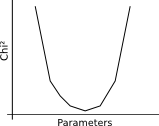
\includegraphics{images/GoodConditioning.png}}
\caption{\label{fig.goodconditioning} Convex, Well-conditioned}
\end{subfigure}
\hfill
\begin{subfigure}{.32\textwidth}
\resizebox{\hsize}{!}{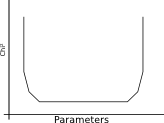
\includegraphics{images/BadConditioning.png}}
\caption{\label{fig.badconditioning} Convex, ill-conditioned}
\end{subfigure}
\hfill
\begin{subfigure}{.32\textwidth}
\resizebox{\hsize}{!}{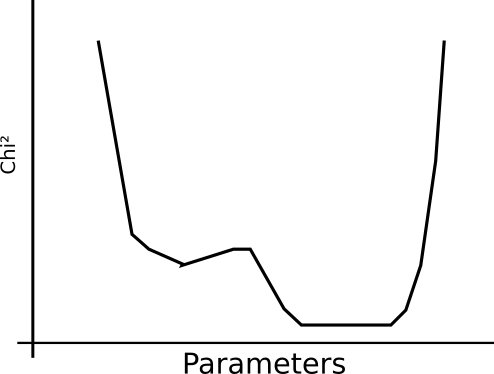
\includegraphics{images/NotConvex.png}}
\caption{\label{fig.notconvex} Non-convex, ill-conditioned}
\end{subfigure}
\caption{\label{fig.examples} Examples of poor conditioning and non-convexity, plotted in terms of residual $\chi^2$ values vs parameter values.  Note that all the parameters of our problem are collapsed onto a single axis and treated as a scalar: this is for illustrative purposes. Note that the local minimum of the non-convex example is well-conditioned while its global minimum is ill-conditioned.}
\end{figure}

\pg
Bad conditioning and non-convexity can be alleviated through regularisation: by specifying a well-chosen prior (e.g. for interferometry, using a good sky model for calibration), the underlying distribution of the solutions can be constrained to fall in a narrow, convex region. This is shown in \cref{fig.selfcal.regularise}
\begin{figure}[h!]
	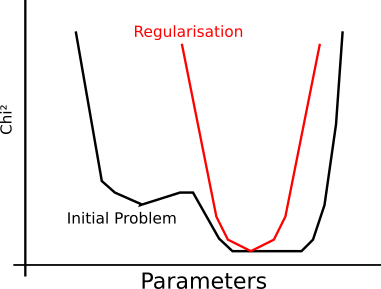
\includegraphics[width=.6\linewidth]{images/regularise.png}
	\caption{\label{fig.selfcal.regularise} Plot showing the effect of regularisation on an ill-conditioned, non-convex problem. The $\chi^2$ fit is constrained to lie in a convex, well-conditioned region: it falls within the global minimum, at at one point only rather than somewhere in a valley.}
\end{figure}

\pg
Because the imaging problem (i.e. the problem of deconvolution) is linear, it can only be convex - though it is not necessarily well-conditioned. As for the calibration problem, experience strongly indicates that it is nearly convex \textit{and} ill-conditioned. For calibration convexity, Cyril Tasse (pers. comm.) has found that the Hessian matrix of the gain solutions is positive semidefinite, i.e. that all its eigenvalues are positive and non-zero except for one. This behaviour likely explains why self-calibration is, in the practical experience of radio-interferometric practicioners,  neither well-conditioned nor convex: if the problem is poorly regularised, then the same initial model may give different end results, and to truly verify the convergence property of self-calibration would require both a full Monte Carlo simulation and enough time to allow the very slowly-converging procedures to finish converging. It is not a practical thing to test rigorously.

\pg
Because the net calibration \& imaging problem has so many degrees of freedom, it is convenient to break it into two parts: calibration and imaging. By doing this, instead of exploring a massive set of hyperparameters (e.g. relative flux distribution at a given frequency, overall spectral index, the 8 values of a complex $2\times 2$ matrix per antenna per time and frequency interval, ...), a smaller subset of these hyperparameters is explored while all else is kept constant. By ensuring that these subsets each give reasonable results individually, it becomes possible to solve the full problem. This practice of imposing specific priors to each subset of the problem is a form of regularisation: it can turn a poorly-conditioned problem into a better-conditioned one, provided that the priors are well-chosen.

\pg
In effect, this means going from exploring the sky-gains parameter space all at once to exploring it along one ``axis\footnote{which includes all the hyperparameters associated with that subset of the problem}" at a time. This is illustrated in \cref{fig.selfcal.paramexplore}. 
\begin{figure}[h!]
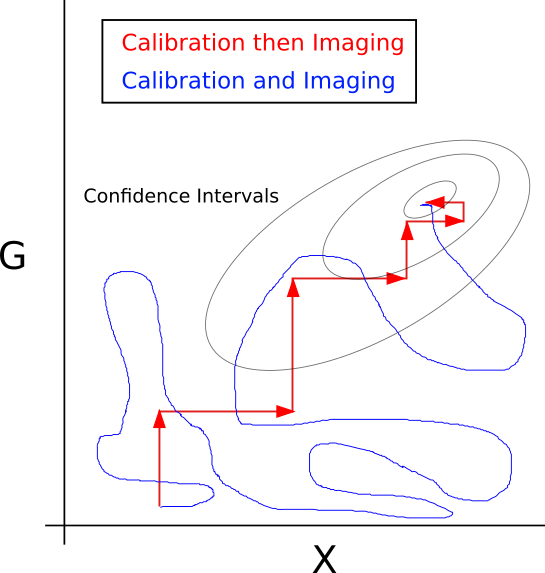
\includegraphics[width=.6\linewidth]{images/Selfcal-paramExplore.png}
\caption{\label{fig.selfcal.paramexplore} Plot showing the exploration of sky-gains (X-G) parameter space. In red, this space is explored one axis at a time (this is ``self-calibration"); in blue, the full space explored at once. Here, we show both procedures converging to the best confidence value: in practice, this is rarely the case.}
\end{figure}

\pg
In this context, a good deconvolution algorithm is one that is able to minimise how much it is affected by calibration errors while maximising how much true underlying flux it can recover into a model, while a good calibration algorithm is one that is able to minimise how much it is affected by sky model errors while maximising how much true underlying gain structure it can recover.



\section{Weighting Schemes}
\pg
We will finish our introduction to the inverse problem of interferometry by discussing one method by which the conditioning of deconvolution can be improved. Consider two extreme cases: a field containing a few point sources(\cref{fig.point}), and a field containing a diffuse and turbulent source, with very complex flux distribution at all scales (\cref{fig.cyga}). Deconvolving the PSF from the first image using CLEAN algorithms will be child's play, but doing the same with the second will be extremely complex. The first case is well-conditioned, and the second to ill-conditioned.

\begin{figure}[h!]
\centering
\begin{subfigure}{.45\textwidth}\resizebox{\hsize}{!}{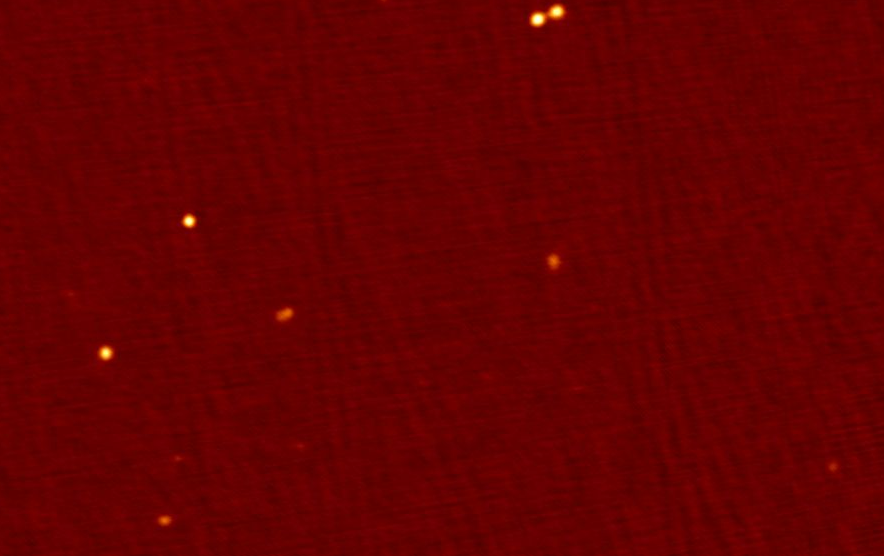
\includegraphics{images/egs-prelim.png}}
\caption{\label{fig.point} Part of the LOFAR field near the Extended Groth Strip as seen by LOFAR.}
\end{subfigure}
\hfill
\begin{subfigure}{.53\textwidth}
\resizebox{\hsize}{!}{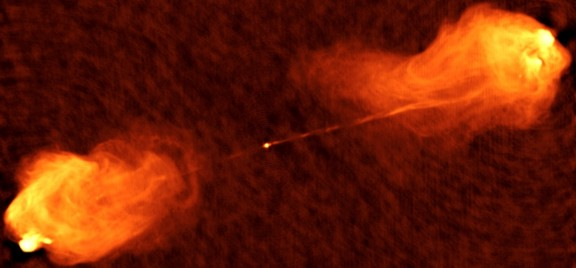
\includegraphics{images/cyga.jpg}}
\caption{\label{fig.cyga} Cygnus A as seen by the VLA. \href{http://images.nrao.edu/110}{Image courtesy of NRAO/AUI}}
\end{subfigure}
\caption{\label{fig.conditioning} Two extreme examples of good and poor conditioning. \cref{fig.point} shows a field with a few point-like sources. \cref{fig.cyga} shows a very complex \& diffuse structure.}
\end{figure}

\pg
The better the conditioning, the easier the deconvolution and the closer to the ground truth its result. As such, when the true underlying structure of a source is poorly-known, getting the best conditioning possible for deconvolution becomes a key concern. Thankfully, because the actual measurements taken with interferometers are the Fourier modes of the sky brightness distribution, they can be weighted when reconstructing the images to fulfill specific requirements. In particular, Briggs weighting \citepads{1995AAS...18711202B} gives a sliding parameter between \emph{natural} weighting, where each visibility is weighed equivalently (this optimises noise in the field) and \emph{uniform} weighting, which gives each visibility a weight inversely proportional to $uv$-plane density. Uniform weighting optimises for resolution at the cost of image signal-to-noise.

\begin{figure}[h!]
\centering
\begin{subfigure}{.48\textwidth}\resizebox{\hsize}{!}{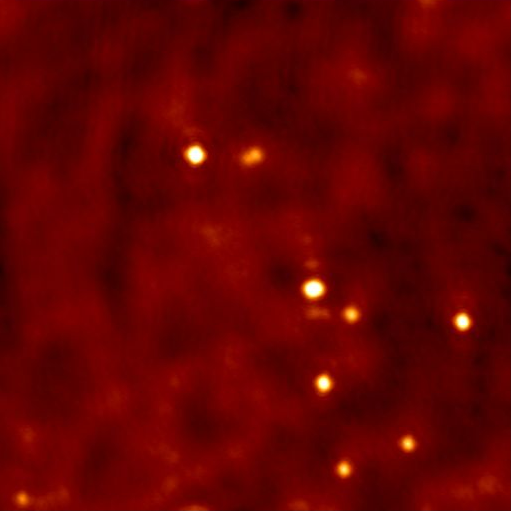
\includegraphics{images/natural.png}}
\caption{\label{fig.natural} Image made with LOFAR data and natural weighting.}
\end{subfigure}
\hfill
\begin{subfigure}{.48\textwidth}
\resizebox{\hsize}{!}{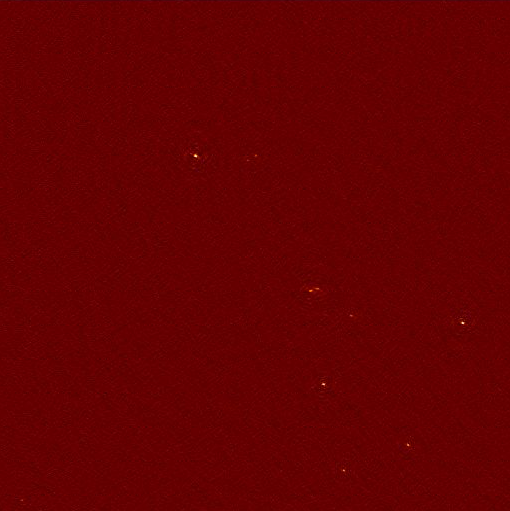
\includegraphics{images/uniform.png}}
\caption{\label{fig.uniform} Image made with the same data as \cref{fig.natural} and uniform weighting.}
\end{subfigure}
\hfill
\begin{subfigure}{.48\textwidth}
\resizebox{\hsize}{!}{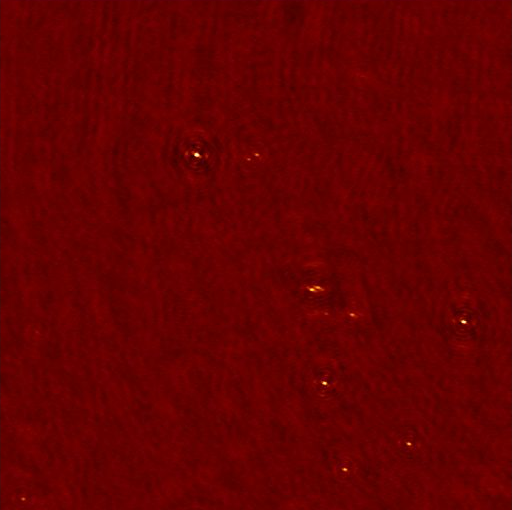
\includegraphics{images/briggs0.png}}
\caption{\label{fig.briggs0} Image made with the same data as \cref{fig.natural} and Briggs weighting, with a Briggs parameter of 0.}
\end{subfigure}
\caption{\label{fig.briggs-weighting}Impact of different weighting schemes on interferometric image reconstruction. All the images shown above are deconvolved.}
\end{figure}

\pg
\cref{fig.briggs-weighting} shows images done with the same data and the same imaging parameters bar weighting scheme choice. We can see that different weighting schemes give radically different deconvolved images. Images made with uniform (\cref{fig.uniform}) or Briggs (\cref{fig.briggs0}) weighing are much sharper, with uniform weighting (\cref{fig.uniform}) giving such resolution that the sources are nearly invisible in the field (though they are present - the contrast was not upped so as to show all three images on the same flux scale). 

\pg
%Note that the weighting schemes shown here rely only on a choice between normalising visibilities by local $uv$-density vs. signal-to-noise, with Briggs weighting providing a formal method for going from one regime to another or optimising between both. Other weighting schemes exist - one can attempt to optimise data size vs decorrelation\footnote{As data is averaged, decorrelation becomes more and more important in the field. See \cref{section.RIME} for more details.}, for example \citepads[see]{2016MNRAS.462.2542A}. This can help ensure a homogeneous conditioning of the deconvolution problem in the image, by ensuring that the PSF is as peaked as possible throughout the field of interest. Part of the work of this thesis was in devising a weighting scheme dependent on calibration quality, to drastically improve deconvolution conditioning and final image quality. This weighting scheme is described in much greater detail in \cref{chapter.paper}.

\pg
We close this section by noting that data flagging can be considered a form of weighting scheme. This consists of assigning a null weight to those data points considered too corrupted by various instrumental or atmospheric effects (typically, Radio Frequency Interference - RFI - cf. \citetads[cf.]{2010ascl.soft10017O} for an example) to be scientifically useful. Those weights which are deemed too corrupted are assigned a weight of zero. This corresponds to simply dropping those data points which would corrupt the image reconstruction by introducing unphysically strong fringes in the image.

\pg
Flagging is also useful to remove corrected visibilities for which near-zero gains are found: the associated corrected visibilities will consist of some number divided by a near-zero number, for which numerical errors can introduce very large errors. ``Clipping" these visibilities after calibration helps improve the final images.

\section{An Observer's Perspective of Radio Interferometry}

\pg
Astronomers who request observation time on interferometric arrays are generally not experts in the theory and operation of these arrays. This is a simple consequence of scientific division of labour. This thesis is written from the perspective of an ``expert" user: one who specialises in understanding interferometric arrays and reducing their data, rather than their subsequent analysis. However, it can be very helpful to contextualise this perspective in the experience of other scientists, which is what this section aims to do. This is simply to highlight the conceptual structure of a radio interferometric observation, and where the concepts outlined in this chapter fall in the overall pattern. In other words, it is best understood as a guide to see where a given section's topic slots into the overall production of an image made from visibilities.

\pg
LOFAR data can be acquired through observation or via the Long-Term Archive. The worst of this data will already be flagged. Users can thus generally proceed directly to calibration. Because there is no guarantee of sufficient signal-to-noise in the ``target field" (the object that the astronomer is actually interested in), it is standard practice to observe a calibrator source for 5 minutes before and after each observation. Such sources typically need to be bright and unresolved for the interferometer being used. Because they are bright and at phase centre for the 5-minute observation, the SNR when solving for calibration solutions for these 5 minutes will tend to be quite good. These solutions will then be interpolated between the 5 minutes onto the 8-hour observation. Calibration will be described in \cref{section.calibration}.

\pg
So far, the astronomer will have worked entirely with visibilities. However, generally speaking, the aim will be to get information on the object's spatial brightness distribution at the observing frequency. This will require \emph{imaging}: going from visibilities to the image-plane. This can be done through a variety of tools, but will generally involve deconvolution. Imaging will be the subject of the rest of this chapter, and deconvolution will be described in more detail in \cref{section.clean}.

\pg
After obtaining the initial image, it may be desirable to perform a few rounds of self-calibration \citepads[cf.]{2018arXiv180505266B} on the target field. This consists of extracting a model from the initial image and using it as a new calibration model, then re-imaging. Doing this will usually dramatically improve the final image. 

\pg
The framework for interferometric calibration is complex, and understanding it requires a good grasp on interferometry itself. For now, we will assume that calibration has been performed perfectly, and that the gain-corrections have been applied to the voltage measured by our antennas. We therefore work with the true signal from astrophysical sources until \cref{section.RIME}.
\clearpage
% !TeX spellcheck = en_UK

\section{Calibration Methods in Radio Interferometry}\label{section.calibration}
\pg
In this section, we will discuss the implementation of interferometric array calibration. Our analysis is based on the RIME formalism, described in \cref{section.RIME}. One key metric of calibration quality is the \emph{dynamic range}, mentioned in Sec. \ref{section.clean}. High dynamic ranges mean that a high contrast has been obtained, and fainter sources can be reached. Here, because the difference between thermal noise and artefacts becomes relevant, we redefine dynamic range as follows
\begin{equation}\label{eq.DR}
DR = \frac{S_{max}}{S_{min},\max(\sigma_{thermal},\sigma_{artefacts})}
\end{equation}
where $S_{max}$ is the flux of the brightest source, $S_{min}$ the flux of the faintest source detectable above the noise, $\sigma_{thermal}$ the thermal noise in the image, and $\sigma_{artefacts}$ the noise associated with calibration artefacts. This gives a definition for dynamic range useful even in fields with a single source. We can thus use it as a metric for calibration quality specifically.

\pg
The distinction between these two noise sources is crucial; one can never go `below noise' for a given observation, no matter the quality of calibration. Astronomers typically observe for longer periods of time in order to reduce $\sigma_{thermal}$ in their images, but this will not reduce the artefacts caused by poor calibration solutions. Uncorrected Direction-Dependent Effects\footnote{See \cref{section.RIME.MultiplePointSources}} will not go away on their own, no matter how long the integration time. Similarly, there is a limit to how much improving calibration will improve the final image: eventually, more data is required to drive noise down.

\pg
We can distinguish three `generations' of calibration methods, of increasing complexity \citepads{2010A&A...524A..61N}. We will describe them in terms of the RIME, showing how each generation increases in generality to account for more exotic effects. They are referred to interchangeably as `nth-generation calibration' or `nGC' methods.

\subsection{Generational Analysis}

\subsubsection{First-Generation: Open-Loop Calibration}\label{section.calibration.1gc}

\pg
First-generation calibration methods (1GC methods) consist of open-loop calibration. This relies entirely on instrument stability, and thus imposes significant design constraints on radio telescopes. It consists of briefly observing an external calibrator before and after each observation run to find calibration solutions for those calibrator observations, and then interpolate between them over the ``target" observation. %\footnote{For a concrete example, see \href{http://www.analog.com/en/analog-dialogue/articles/open-loop-calibration-techniques.html}{the open-loop calibration techniques page of analog.com}.}
%\pg
%Phase calibration in the 1GC era `proper' was not necessary, as engineers were capable of ensuring adequate phase stability in contemporary interferometers. Phase was thus calculated relative to a fixed frame of reference, usually the central antenna of a 3-antenna array. 
In RIME terms (see \cref{section.RIME}), this consists of solving for a very basic form of $\Gjones_p$:
\begin{equation}
\Gjones_p = a_p \bm{\mathrm{I}} % \begin{bmatrix} e^{2 \pi i \nu ( \phi_p - \phi_0)} \end{bmatrix}
\end{equation}
where $a_p$ is a complex constant solved for during open-loop calibration. By interpolating between the two calibrator observations, it is possible to have a linear time-dependent gain estimate, though it is not much more complex than the above. %, $\nu$ the observing frequency, $\phi$ the phase at an antenna, and $\phi_0$ the phase at the reference antenna.

\pg
While values for $a_p$ and $b_p$ can in theory be found for both autocorrelation and both crosscorrelations (e.g. XY and YX for linear receptors), low signal-to-noise means that in practice, a single set of values is solved for per antenna\footnote{This reduces calibration to solving only for the intensity gains: the data can then only be used for \emph{intensity mapping} (e.g. \citepads{1957IAUS....4..159J}). This practice therefore precludes polarimetry.}. With these techniques, one can achieve dynamic ranges of about 100:1 (\citepads{2010A&A...524A..61N}).

\subsubsection{Second-Generation: Self-Calibration}\label{section.calibration.2gc}

\pg
Second-generation calibration methods (2GC methods) are defined by \emph{self-calibration}\footnote{On the discovery of self-calibration and its evolution in parallel to adaptive optics, see the chapter titled "The Almost Serendipitous Discovery of Self-Calibration'' in "\href{http://library.nrao.edu/public/collection/02000000000280.pdf}{\citep{serendipitous}}.}, commonly referred to as \emph{self-cal} (\citepads{1984ARA&A..22...97P}). As described in \cref{section.RIME.FullSky.CVZ}, this method can only be deployed if the brightness matrix of the sky is the same for all baselines\footnote{This is not to say that the brightness matrix must contain only point sources, but rather that moving our interferometer 500m to the East should not change its measured visibilities} (i.e. that we are not affected by direction-dependent effects).

\pg
The first instance of self-calibration (and adaptive optics in radio interferometry) is a paper published in the era of 1GC by Jennison \citepads{1958MNRAS.118..276J}, expanding on his PhD work, which was published in 1951). With sufficient signal-to-noise, he showed that \emph{phase closure} could be calculated and errors due to the atmosphere thus mitigated.

\pg
Self-calibration and adaptive optics are essentially the same thing, albeit meeting different constraints. Most notably, interferometric data is digital, allowing radio astronomers to perform their adaptive optics correction after the observation.

\pg
If amplitude and phase gains can be written as antenna-dependent, then each antenna-based error is estimated N times (once per each baseline which includes this antenna). By estimating, and correcting for, these errors, one can use a simple source model to infer an improved one. This is why the method is referred to as self-cal; by calibrating `on' a good calibrator source (bright, compact and unresolved), one can drastically improve one's source model, along with one's calibration solutions.


\begin{figure}[h!]
\centering
\resizebox{\hsize}{!}{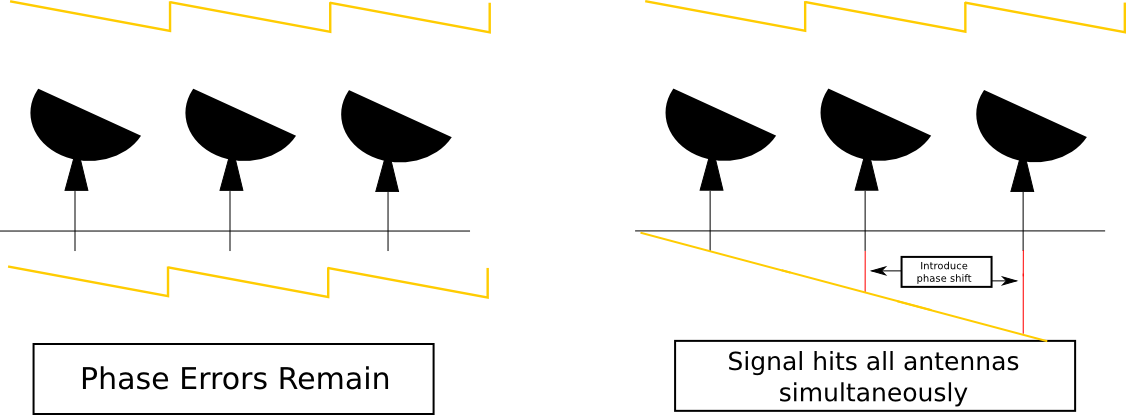
\includegraphics{images/selfcal.png}}
\caption{\label{fig.selfcal} Representation of self-calibration as adaptive optics}
\end{figure}

\pg
By extending this idea to VLBI (see e.g.  \citepads{1974ApJ...193..293R}), \emph{amplitude closure} was introduced to the field along with phase closure \citepads[as described in][]{1983Sci...219...51R}. These quantities are immune to antenna-based effects.%Astronomers were quick to apply these methods to interferometers in general.

\pg
The great advantage of radio interferometry over optics, however, is that we can \emph{iterate} over progressively improved source models. This is because interferometric data is digital, and because we record phase information.

\pg
In practice, of course, self-cal will be limited by noise. More precisely, it will be limited by two factors: sensitivity, in the form of the signal-to-noise ratio (henceforth SNR), and the atmosphere (as sufficient SNR is needed per coherence time, which is a function of atmosphere activity). For sufficiently bright sources, with high SNR, self-calibration can easily improve dynamic range by a factor of 10 (\cite{serendipitous}, p. 154) in a single iteration. 

\subsubsection{Third-Generation: Direction-Dependent Effects}

\pg
Third-generation calibration (3GC) is an extension of 2GC calibration which takes direction-dependent effects into account. At the time of writing, this is the cutting edge in radio interferometric calibration.

\pg
In this section, I will discuss the \emph{facet-based} approach taken by \citetads{2017arXiv171202078T}. The approach cannot be divorced from imaging, for the simple reason that solving for and applying Jones matrices\footnote{See \cref{section.RIME} for a full discussion on calibration and Jones matrices} in different directions requires image-plane knowledge of the sky brightness distribution $\Bmatrix$. % The imaging challenges this methods introduces will be discussed in [href to relevant imaging section].

\begin{figure}[ht]
\centering
\resizebox{\hsize}{!}{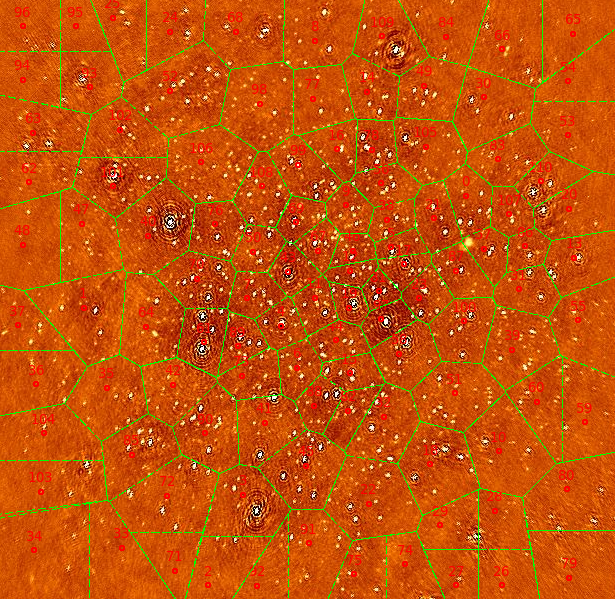
\includegraphics{images/bootes-image.png}}
\caption{\label{fig.facets} Voronoi facets, as implemented in DDFacet. Image is made before application of direction-dependent correction. This is an image of the Bootes field, made by Cyril Tasse.}
\end{figure}

\pg
When performing first and second-generation calibration, one solves for a set of Jones matrices or parameters thereof. Direction-independent calibration then consists of applying these calibration solutions to the visibilities directly. However, while these solutions will be correct in the direction of the calibrator source, they are increasingly likely to be wrong as a function of distance from said calibrator source. The difference between the true gains in a given direction and the gains estimated from the calibrator source are called \emph{differential gains}.

\pg
Why then not solve for a set of calibration solutions for each source in the calibration model, iteratively adding new sources to this model as they become above the noise as calibration artefacts - introduced by poor calibration - decrease? There are two main reasons for this: firstly, the SNR when calibrating using very faint source models will be poor. This means that gains will likely be extremely noisy, and applying them will result in increased calibration artefacts in the final image. Secondly, even by optimising for signal-to-noise and only using a few of the brightest sources in the field, the problem quickly becomes intractably large in terms of computing power required, provided that standard complex differentiation is used \citepads[see][]{2016ApJS..223....2V}. Wirtinger differentiation \citepads[see][]{2014arXiv1410.8706T,2015MNRAS.449.2668S} does alleviate this somewhat by allowing the Hessian matrix to be written as a block-diagonal matrix, but is not implemented in all standard direction-dependent calibration software at the time of writing.

\pg
The crucial insight of a faceting approach is then to split the image into a set of \emph{facets}, solving for a set of calibration solutions for each of these facets. These solutions are then applied to the visibilities when mapping them onto the dirty image. The faceting in DDF is shown in \cref{fig.facets}. The facet distribution shown in \cref{fig.facets} encourages an even flux distribution in multiple facets, and ensures that no facet is so small that too little signal would be available within. As we can see from \cref{fig.DDcal.effect}, direction-dependent calibration can drastically improve the quality of wide-field images. It currently represents the state of the art in interferometric calibration. 

\begin{figure}[h!]
\centering
\begin{subfigure}{\textwidth}
\resizebox{\hsize}{!}{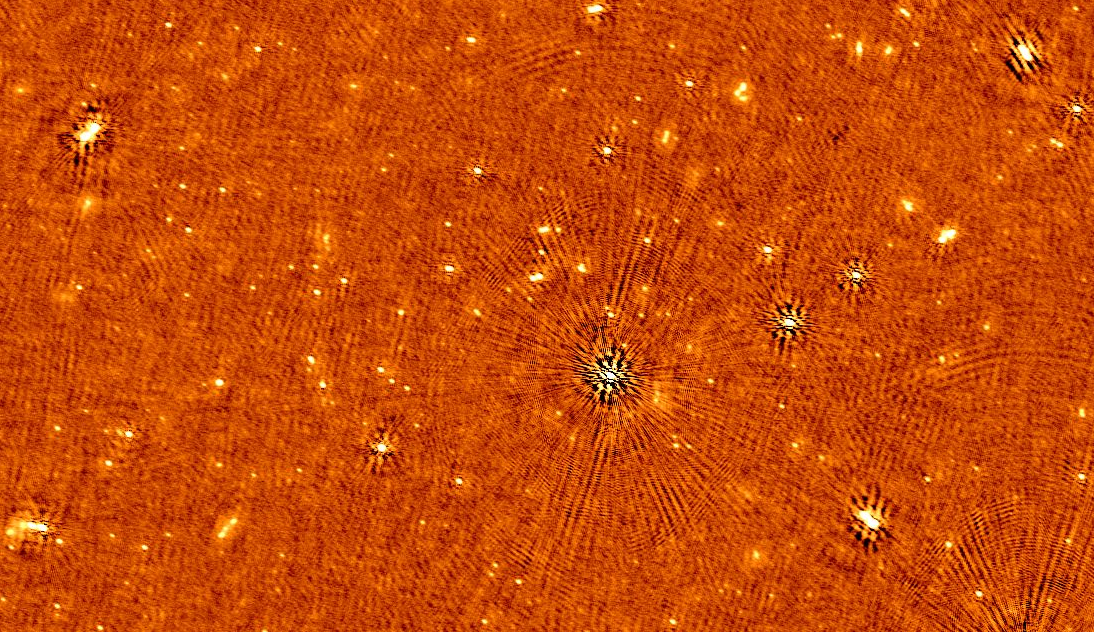
\includegraphics{images/lofar-nocorr.png}}
\caption{\label{fig.lofar.noDDcal} Image of the Boötes field, made without direction-dependent calibration. Image by Cyril Tasse.}
\end{subfigure}
\begin{subfigure}{\textwidth}
\resizebox{\hsize}{!}{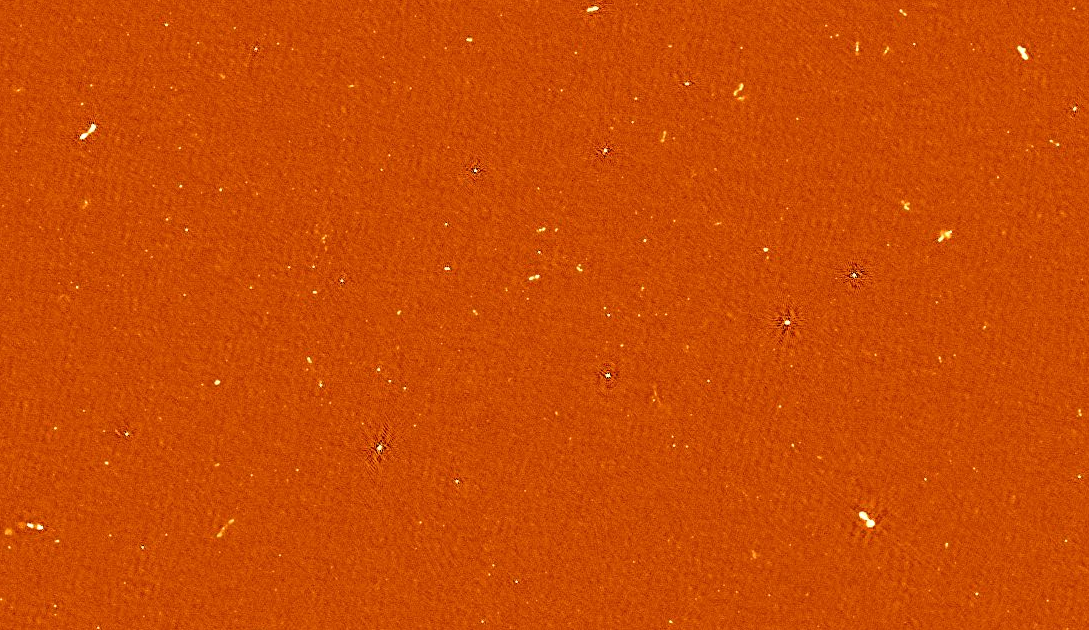
\includegraphics{images/lofar-corr.png}}
\caption{\label{fig.lofar.withDDcal} Image of the same Boötes field, made with direction-dependent calibration. Image by Cyril Tasse.}
\end{subfigure}
%\hfill
\caption{\label{fig.DDcal.effect} Difference between imaging made with (Fig. \ref{fig.lofar.withDDcal})and without (Fig. \ref{fig.lofar.noDDcal}) third-generation calibration.}
\end{figure}








\clearpage
% !TeX spellcheck = en_UK

\section{The RIME Formalism}\label{section.RIME}
%\minitoc

\pg
In this section, we introduce the mathematical framework which forms the basis for our algorithmic work.
While radio interferometry has historically been a complex business \citepads{2001isra.book.....T}, modern radio interferometry is based on the Radio Interferometer's Measurement Equation, a powerful and elegant formalism which underpins modern calibration and imaging algorithms. In this section, I will give a simplified account of this formalism as described in \citetads{2011A&A...527A.106S} and its companion papers \citepads{2011A&A...527A.107S, 2011A&A...527A.108S, 2011A&A...531A.159S}. This will form the theoretical basis on which further sections will expand.% I cannot overstate the importance of the RIME as the foundation of modern calibration and imaging algorithms.

\pg
For a mathematically rigorous description of the RIME, the references used in this work (particularly \citetads{2011A&A...527A.108S} and \citetads{2011A&A...531A.159S}) are obviously the first place to look. We frame the RIME in the continuity of previous theoretical frameworks of radio interferometry, while also describing it in the context of contemporary software packages and algorithmic tools.

\section{Setting up the RIME: a single point source}
\label{section.RIME.setup}

\pg
The Radio Interferometer's Measurement Equation, or RIME, is a formalism which allows for an elegant and efficient formulation of the physical processes which affect signal propagation, from astrophysical effects to instrumental effects. Its fundamental underlying hypothesis is \emph{linearity}: that transformations along the signal are linear with respect to the basis chosen to represent our signal. In other words, this means assuming that propagation effects are separable by antenna.

\pg
Consider a single quasi-monochromatic point source in the sky. Its signal at a point in time and space can be described by a complex 2-vector $\evector$ -- this assumes plane waves. We can then represent physical processes which affect this signal's propagation using \emph{Jones matrices}. In other words:
\begin{align}
\volt &= \Jones\evector\\
\evector &= \begin{pmatrix} e_x \\ e_y \\ e_z \end{pmatrix}
\end{align}
where $\volt$ is the voltage measured by our antenna, and $\Jones$ the Jones matrix describing the \emph{net} propagation effects - atmospheric, astrophysical, and instrumental - which affect our source's signal. $\evector$ is the electromagnetic wave emitted by a source. $\Jones$ can be written as a series of matrix products, each individual matrix describing a physical phenomenon. They are then called a \emph{Jones chain}, and the resulting $\Jones$ is often called the \emph{total Jones matrix}.

\pg
For $\mathbf{e}$ to be a 2-vector, rather than a 3-vector, we must choose to use $xyz$ as our coordinates, with $z$ the direction of propagation of our signal. \citetads{1996A&AS..117..137H} then show that the following relation holds:
\begin{equation}
2 \evector \evector^\Herm = 2  \begin{bmatrix} <e_x e_x^\star> & <e_x e_y^\star> \\ <e_y e_x^\star> & <e_y e_y^\star> \end{bmatrix} = \begin{bmatrix} I+Q & U+iV \\ U-iV & I-Q \end{bmatrix} = \Bmatrix
\end{equation}
where $\Bmatrix$ is the coherency matrix of the source's emission.

\pg
A visibility is the correlation of voltage from two antennas. In other words,
\begin{align}
\Vis_{pq} &= 2 \langle\volt_p (\volt_q)^\Herm\rangle\\
\Vis_{pq} &= 2 \langle\Jones_p \evector (\Jones_q \evector)^\Herm\rangle\\
\Vis_{pq} &= 2 \langle\Jones_p \evector \evector^\Herm \Jones_q^\Herm\rangle
\end{align}
where $\Jones_p$ corresponds to the signal propagation chain of antenna $p$, and $\Jones_q$ for antenna $q$. $(...)^\Herm$ corresponds to taking the Hermitian conjugate of a matrix, and $\langle...\rangle$ an average over some interval. Note that a factor of 2 has been introduced here, as a matter of convention. This is due to the definition of the Stokes parameter in relation to our $\evector$ outer product.



\pg
We can thus write:
\begin{equation}
\Vis_{pq} = \Jones_p \Bmatrix \Jones_q^\Herm
\end{equation}

\pg
This gives us an elegant formulation of the relationship between the signal emitted by an astrophysical source and its corresponding measured visibility. The Stokes parameters\footnote{Stokes parameters determine the polarisation of light; we will not get into more details in this manuscript, as it is hardly relevant to the topic at hand. Suffice to say that the 2-vector formalism helps account for the polarised nature of light.} of our source can be directly calculated from our measured visibility, provided $\Jones_p$ and $\Jones_q$ are known. Of course, in practice, they are not, and must therefore be modelled. To do this, we must expand each Jones matrix into a corresponding Jones chain.

\section{Expanding our Jones Chain}
\label{section.RIME.JonesChain}
\pg
Having written our RIME as a matrix multiplication problem, we can now begin to differentiate between different types of Jones matrices. $\Jones_p$ describes the \emph{aggregate} effects which occur over the course of the signal's propagation to our antenna $p$. It can be split into a Jones chain of $n$ separate matrices, corresponding to different effects:
\begin{align}
\displaystyle \Jones_{sp}^H &= \prod_1^n \Jones_{nsp}^H = \Jones_{1sp}^H \Jones_{2sp}^H ... \Jones_{nsp}^H\label{eatshit1}\\
\displaystyle \Jones_{sp}   &= \Jones_{nsp}...\Jones_{2sp} \Jones_{1sp}\label{eatshit2}
\end{align}
where $s$ is a particular direction in the sky: these Jones matrices are therefore direction-dependent. Going from \cref{eatshit1} to \cref{eatshit2} simply consists of applying the Hermitian operator to both sides of \cref{eatshit1} to recover $\Jones_{nsp}$.
Since the Jones terms are applied sequentially to the brightness matrix, starting with $\Jones_{1sp}$, the terms to the right of our decomposition of $\Jones_{sp}$ can be said to occur `at the source', i.e. before those to the left (said to occur `at the antenna').

\pg
Our aim is thus to find the Jones chain which most concisely describes the different \emph{types} of effects affecting our signal. In order of increasing complexity, there are three: so-called \emph{geometric} effects, \emph{direction-independent} effects, and \emph{direction-dependent} effects.

\subsection{Geometric Effects: the Phase Delay Jones Matrix}
\label{section.RIME.JonesChain.Kjones}

\pg
The physical quantity measured by an interferometric array, the \emph{visibility}, is not a function of the absolute phase of our signal, but rather a function of the \emph{phase difference} between our measured voltages $\volt_p$ and $\volt_q$. In other words, it is a function of the phase difference on \emph{baseline} $pq$, which consists of antennas $p$ and $q$. The direction which minimises this difference is called the \emph{phase centre}\footnote{Bear in mind the limitations of this, described in \cref{sec.visibility}.}.

\pg
We shall use the conventional coordinate system and notations \citepads[][etc]{2011A&A...527A.106S,2001isra.book.....T}. We thus have a $z$ axis pointing towards the phase centre, and an antenna $p$ at coordinates $\U_p=(u_p,v_p,w_p)$. The phase difference between $p$ and phase centre (where, by definition, $\U=0$) for a signal arriving from direction $\pmb{\sigma}$ is then, assuming a small field of view:
\begin{equation}
k_p=2\pi i (( u_p l + v_p m + w_p (n-1) ))
\end{equation}

where $n=\sqrt{1-l^2-m^2}$. Here, $l,m,n$ are the direction cosines\footnote{The $n-1$ term in the exponential is due to the fact that, at phase centre, $k_p=0$ for all $\U$ and $n=\sqrt{1-0-0}=1$.} of $\pmb{\sigma}$, and $\U$ is defined in units of wavelength\footnote{This means that, for a given baseline $pq$, $\U$ will vary as a function of frequency.}.

\pg 
Having done this, we can now introduce a scalar \emph{K-Jones} matrix to represent the effect of this phase delay. Since it is scalar, it will commute with all other Jones matrices \citepads[see]{2011A&A...527A.106S}. It can be be written as:
\begin{equation}
\Kjones_p = e^{-i k_p}  = e^{-2\pi i ( u_p l + v_p m + w_p (n-1) )}
\end{equation}

\subsection{The Coherency Matrix}
\label{section.RIME.JonesChain.CoherencyMatrix}

\pg
The commutation property of $\Kjones_p$ with other Jones matrices allow us to always place it at the rightmost end of our Jones chain. We can thus write our Jones chain as follows:
\begin{align}
\Jones_p  &= \Gjones_p \Kjones_p\\
\end{align}

\pg
Here, we have decoupled the nominal phase delay term ($\Kjones_p$) from all `corrupting' effects ($\Gjones_p$). We can take this one step further by defining the \emph{source coherency}, $\Coherency_{pq}$, as follows:
\begin{align}\label{eq.def.coherency}
\Coherency_{pq} &= \Kjones_p \Bmatrix \Kjones_p^H\\
\Vis_{pq} &= \Gjones_p \Coherency_{pq} \Gjones_q^H
\end{align}

\pg
This is useful on a conceptual level: the process of \emph{calibration} is now to find a best estimate for $\Gjones_p$, which contain all non-`geometric' physical effects on the signal's propagation from an astrophysical source to our voltage measurement.

\pg
On a practical level, using the coherency matrix $\Coherency$ allows us to write our RIME more concisely, by absorbing the geometric effects into the core of our RIME. While not strictly necessary, it can be a useful thing to do.

\section{Multiple Point Sources}
\label{section.RIME.MultiplePointSources}

\pg
So far, $\Bmatrix$ represents the signal from a single point source. However, the formalism can be extended to multiple point sources. This is because electric fields -- and therefore radio signals -- are additive, and that signal from different sources is not coherent (see \cref{eq.spatial.incor}), which means that visibilities are additive. If our sky contains $s$ point sources, then our RIME becomes:
\begin{equation}
\Vis_{pq} = \sum_s \Jones_{sp} \Bmatrix_s \Jones_{sq}^\Herm
\end{equation}

\pg
We now expand our Jones chain as before. Some, but not all, elements in the chain will only depend on the antenna. These will be the same for all sources. We can thus write our Jones chain as:
\begin{equation}
\Jones_{sp} = \Gjones_p \Ejones_{sp} \Kjones_{sp}
\end{equation}
where $E_{sp}$ are direction-dependent effects, which vary for each source. Note that we have kept the source-dependent effects (i.e. those which vary depending on the line of sight) are to the right of our chain, and the antenna-dependent ($G_p$) effects to the left. $K_{sp}$ is a scalar and can thus be moved at will; it is therefore placed at the far right to recover the coherency matrix if necessary.

\pg
Our multiple-source RIME can thus be written in the following form:
\begin{equation}\label{eq.multiple.source.RIME}
\Vis_{pq} = \Gjones_p \bigg( \sum_s \Ejones_{sp} \Kjones_{sp} \Bmatrix_{s} \Kjones_{sq}^H \Ejones_{sq}^H \bigg) \Gjones_q^H
\end{equation}

\pg
This `onion' form of the RIME - so-called because, like an onion, it is formed in layers - is usually sufficient to describe signal propagation in radio-interferometric arrays. We find the three types of Jones matrices promised earlier: the geometric effects accounted for by $\Kjones$, the direction-dependent effects modeled into $\Ejones$, and the direction-independent effects (antenna-based effects) modeled into $\Gjones$.

\pg
There are still limitations to this RIME; notably, it assumes that the sky consists entirely of point sources (absence of diffuse emission), and that Jones matrices are time-independent. These are of course unphysical hypotheses, though they are a very good first approximation. We shall now address these two points.

\section{Diffuse Emission: the Full-sky RIME}
\label{section.RIME.FullSky}

\subsection{Deriving the Fully-Sky RIME}
\label{section.RIME.FullSky.derivation}
\pg
If we want to be able to take diffuse emission properly into account, we must go from our set of discrete point sources $\Bmatrix_s$ and integrate the underlying continuous brightness distribution $\Bmatrix(\direction)$ over all possible directions. This gives us the following expression:
\begin{equation}
\Vis_{pq} = \int_{4\pi} \Jones_p(\direction) \Bmatrix(\direction) \Jones_q^H(\direction)d\Omega
\end{equation}

\pg
Here, effects such as our array's beam lie in the Jones matrices. By performing the analysis shown in Sect. 3.1 of \citetads{2001isra.book.....T}, we can rewrite this expression in terms of a sine projection of the sphere onto the $(l,m)$ plane tangential at field centre. The integral then becomes:
\begin{equation}
\Vis_{pq} = \int_{l,m} \Jones_p(\direction) \Bmatrix(\direction) \Jones_q^H(\direction)\frac{dl dm}{n}
\end{equation}

\pg
Having written this, and using $\lvec$ as shorthand $(l,m)$, we can once again decompose our Jones matrix into a Jones chain containing a direction-independent term $\Gjones$, a direction-dependent term $\Ejones$, and the phase term $\Kjones$. Substituting this into our integral, we get the following expression:
\begin{align}
\Vis_{pq} &= \Gjones_p \bigg(\int_{\lvec} \frac{1}{n} \Ejones_p(\lvec) \Kjones_p(\lvec) \Bmatrix \Kjones_q^H(\lvec) \Ejones_q(\lvec)  dl dm \bigg) \Gjones_q^H\\\Vis_{pq} &= \Gjones_p \bigg(\int_{\lvec} \frac{1}{n} \Ejones_p(\lvec) \Bmatrix \Ejones_q(\lvec) \Kjones_p(\lvec)\Kjones_q^H(\lvec) dl dm \bigg) \Gjones_q^H\\
          &= \Gjones_p \bigg(\int_{\lvec} \frac{1}{n} \Ejones_p(\lvec) \Bmatrix \Ejones_q(\lvec) e^{-2\pi i\big(u_{pq}l+v_{pq}m+w_{pq}(n-1)\big)} dl dm \bigg) \Gjones_q^H
\end{align}
where
\begin{alignat}{3}
u_{pq}&=u_p-u_q \qquad v_{pq}&=v_p-v_q \qquad w_{pq}&=w_p-w_q
\end{alignat}

\pg
This is a three-dimensional Fourier transform. It can be reduced to a two-dimensional Fourier transform by writing the $n$-dependence in the exponential (and normalisation) as a Jones matrix, thus removing the \emph{non-coplanarity} terms from the explicit RIME. We can thus define the following:
\begin{align}
\Wjones_p &= \frac{1}{\sqrt{n}}e^{-2\pi i w_p(n-1)}\\
B_{pq}    &= \Ejones_p \Wjones_p \Bmatrix \Wjones_q^H \Ejones_q^h
\end{align}
and write our RIME in its final form:
\begin{equation}\label{eq.vis.FT.coherency.matrix}
\Vis_{pq} = \Gjones_p \bigg(\int_{\lvec} \Bmatrix_{pq}(\lvec) e^{-2\pi i\big(u_{pq}l+v_{pq}m+w_{pq}(n-1)\big)} dl dm \bigg) \Gjones_q^H
\end{equation}
\pg
Note that $\Bmatrix$ was the actual sky  brightness distribution as a function of direction, but now $\Bmatrix_{pq}$ is the sky brightness \emph{as seen by baseline pq} -- in the presence of direction-dependent effects, this is not the same for all baselines.\\

\subsection{Recovering the van Cittert-Zernike Theorem}
\label{section.RIME.FullSky.CVZ}

\pg
Earlier calibration models and algorithms rely on the hypothesis that all baselines see the same sky. This is the \emph{fundamental premise of self-calibration}. The topic of self-cal is covered in \cref{section.calibration.2gc}. This premise only holds when all Direction-Dependent Effects (henceforth referred to as DDEs) are identical for all baselines (and therefore for all antennas). We then effectively have $\Ejones_{s,p}=1$ for all $p$. This is a necessary condition for the \textit{apparent} sky $\Bmatrix_{pq}$ to be the same for all baselines\footnote{The ``apparent" sky is the `true' sky attenuated by the ``power beam", which corresponds to our instrument's directional sensitivity in the traditional view.}, as it allows us to write:
\begin{align}
\Ejones_p(\lvec) \Wjones_p(\lvec)&= \Ejones(\lvec) \Wjones(\lvec)\\
\Bmatrix_{pq}(\lvec) = \Bmatrix_{app}(\lvec) &= \Ejones(\lvec) \Wjones(\lvec) \Bmatrix (\lvec) \Wjones^H(\lvec) \Ejones^H(\lvec)
\end{align}

\pg
If this condition is met, we can then rewrite the full-sky RIME as:
\begin{equation}\label{eq.fullsky.RIME}
\Vis_{pq} = \Gjones_p \Coherency_{pq} \Gjones_q^H
\end{equation}
where $\Coherency_{pq} = \Coherency(u_{pq},v_{pq}) = \Coherency(\uvec)$. Our coherency matrix includes the beam attenuation implicitly, as $\Bmatrix_{app}$ is now the coherency of the \textit{apparent} sky brightness distribution. Comparing \cref{eq.def.coherency,eq.vis.FT.coherency.matrix} directly shows that the coherency matrix is simply the two-dimensional Fourier transform of $\Bmatrix_{app}(\lvec)$. We can thus call $\Coherency(\uvec)$ the \emph{sky coherency}, in keeping with our nomenclature for the RIME of a point source.

\pg
Note that deriving the van Cittert-Zernike theorem (\citepads{1934Phy.....1..201V}, covered in \citepads{2001isra.book.....T}) from the RIME was simply of matter of treating phase as a Jones matrix in its own right\footnote{\href{https://raw.githubusercontent.com/wiki/ska-sa/meqtrees/aips++_note185.pdf}{Noordam, J.E. 1996, AIPS++, Note 185: The Measurement Equation of a Generic Radio Telescope}}. A significant consequence of this is that DDEs can be incorporated within the RIME formalism.

\section{Time-dependent Jones matrices, Smearing, and Decorrelation}
\label{section.RIME.TimeDep}

\subsection{Time-dependence of Jones matrices}
\label{section.RIME.TimeDep.Jones}

\pg
Until this point, we have not considered any kind of sky variability in time. In effect, \cref{eq.fullsky.RIME} describes the snapshot taken by an interferometer for a single measurement. Limiting ourselves to this scenario, however, strongly limits the sampling of the $uv$-plane which can be performed. Indeed, interferometers generally rely on the Earth's rotation to rotate their baselines $pq$, thus increasing $uv$-coverage at no additional cost.This technique is known as \emph{super-synthesis} (\cite{supersynthesis}\footnote{\href{http://www.jpier.org/PIERB/pierb22/05.10032105.pdf}{\url{http://www.jpier.org/PIERB/pierb22/05.10032105.pdf}}}) For \cref{eq.fullsky.RIME} to hold throughout an observation, we must therefore assume that $B_{app}$ remains constant in time over the course of the observation. In effect, this means assuming that
\begin{equation}\label{eq.selfcal.requirement}
\Ejones_p(t,\lvec) = \Ejones_p(\lvec) = \Ejones(\lvec) \quad \forall (t,p)
\end{equation}

\pg
The above means that direction-dependent effects must be time-independent for \cref{eq.fullsky.RIME} to hold. We can thus split direction-dependent effects into two categories: \emph{trivial} DDEs, which satisfy this condition and are a simple multiplicative correction, and \emph{non-trivial} DDEs, which are not. An example of a trivial DDE is the primary gain; and example of a non-trivial (i.e. time-variable) DDE is ionospheric turbulence.

\subsection{Smearing and Decorrelation}
\label{section.RIME.TimeDep.Decoherence}

\pg
Of course, our Jones matrices are not the only time-dependent element of the RIME formalism. As mentioned above, to image with interferometric arrays, radio astronomers rely on the Earth's rotation to better sample $uv$-space. This means that $\uvec$ becomes a \emph{time-dependent} variable.

\pg
Furthermore, if we choose to define $\uvec$ in terms of wavelength, $\uvec_p$ becomes dependent in frequency. Our time-independent, frequency-independent RIME thus becomes only valid for infinitesimal increments in time and frequency.

\pg
In practice, measurements made by any interferometric array are actually averaged over the integration time of the measurement, as well as the frequency channel size. A better formulation is therefore to explicitly write the RIME as an integration over time and frequency bins:
\begin{align}
\langle \Vis_{pw} \rangle &= \frac{1}{\Delta t \Delta \nu} \int_{t_0}^{t_1} \int_{\nu_0}^{\nu_1} \Vis_{pq}(t,\nu) dv dt\\
                          &= \frac{1}{\Delta t \Delta \nu} \int_{t_0}^{t_1} \int_{\nu_0}^{\nu_1} \Jones_p(t,\nu) \Bmatrix \Jones_q^H(t,\nu)
\end{align}

\pg
$\Jones(t,\nu)$ describes the propagation of an electromagnetic signal through various physical processes. This signal has a complex phase, which is variable in both time and frequency. Since it is a rotating vector, integrating over any time or frequency band will always result in a \emph{net loss} in amplitude in the measured $\langle\Vis\rangle$. This mechanism is commonly referred to as \emph{time/bandwidth decorrelation} or \emph{smearing} \citepads{2011A&A...527A.106S}.

\pg
The general effect is referred to as \emph{decorrelation}\footnote{Decorrelation can equivalently be referred to as ``decoherence".}, and the specific case of decoherence caused by the $\Kjones$ term is referred to as \emph{smearing}.

\pg Smearing increases with baseline length ($\uvec_{pq}$) and distance from phase centre ($l,m$). The noise amplitude, however, does not decrease. This means that smearing results in a decrease in sensitivity, which becomes significant when attempting to do wide-field, high-resolution images (see \cref{section.decorr}).

\pg 
In the context of the RIME, smearing is an element-by-element operation, i.e. different elements do not affect each other. Treating smearing within the RIME is thus a trivial expansion of the scalar equations.

\pg
Assuming that $\Delta t$ and $\Delta \nu$ are small enough that the amplitude of $\Vis_{pq}$ remains constant over the integration band (i.e. that $\Vis_{pq}$ is well-sampled by our instrument), then a useful first-order approximation\footnote{see \citetads{2011A&A...527A.107S} and companion papers.} is:
\begin{equation}
\langle \Vis_{pw} \rangle \simeq \text{sinc}\frac{\Delta \pmb{\Psi}}{2} \enskip \text{sinc}\frac{\Delta \pmb{\Phi}}{2} \enskip \Vis_{pq}(t_{mid},\nu_{mid})
\end{equation}
where
\begin{align}
t_{mid}           &= (t_0 + t_1)/2\\
\nu_{mid}         &= (\nu_0 + \nu_1)/2
\end{align}
\begin{align}
\Delta \pmb{\Psi} &= \arg \Vis_{pq}(t_1,\nu_{mid}) - \arg \Vis_{pq}(t_0, \nu_{mid})\\
\Delta \pmb{\Phi} &= \arg \Vis_{pq}(t_{mid},\nu_1) - \arg \Vis_{pq}(t_{mid}, \nu_0)
\end{align}

\pg
This equation is convenient to determine the impact of decorrelation for a source at a given distance from phase centre. Note, however, that it can only - by definition - be valid for a single source at a time. If using a RIME such as \cref{eq.multiple.source.RIME}, then it can be calculated for each source individually.

\section{Noise}
\label{section.RIME.noise}

\pg
The RIME presented thus far has been for an ideal case, free of noise in our measured visibility. In practice, each complex visibility will be affected by uncorrelated Gaussian noise\footnote{Detailed treatment given in \citepads{2001isra.book.....T}, section 6.2, which shows how to obtain the ideal radiometer equation}, which means that a RIME of the same form as \cref{eq.multiple.source.RIME} would have to be formuled at follows:
\begin{equation}
\Vis_{pq} = \Gjones_p \bigg( \sum_s \Ejones_{sp} \Kjones_{sp} \Bmatrix_{s} \Kjones_{sq}^H \Ejones_{sq}^H \bigg) \Gjones_q^H + \sigma_{pq}
\end{equation}
where $\sigma_{pq}$ is a $(2,2)$ matrix with real and complex parts in each component. A similar addition can be made for any of the RIMEs presented here.

\pg
This noise sets a hard limit on the sensitivity achieved for a given observation, and `reaching the noise' becomes the gold standard of calibration \citepads{2011A&A...527A.107S}. One must then take $\sigma_{pq}$ into account properly when solving for the Jones matrices.



